\documentclass[12pt]{article}

\usepackage{amsmath}
\usepackage{graphicx}
\usepackage{amsfonts}
\usepackage{amsthm}
%\usepackage{cite}
\usepackage{times}
\usepackage{geometry}
\usepackage[round,numbers,sort&compress]{natbib}
\oddsidemargin=0.0in %%this makes the odd side margin go to the default of 1inch
\evensidemargin=0.0in
\textwidth=6.5in
\textheight=9in %%sets the textwidth to 6.5, which leaves 1 for the remaining right margin with 8 1/2X11inch paper

\providecommand{\ve}[1]{\boldsymbol{#1}}
\providecommand{\norm}[1]{\left \lVert#1 \right  \rVert}
\providecommand{\deter}[1]{\lvert #1 \rvert}
\providecommand{\abs}[1]{\lvert #1 \rvert}
\providecommand{\tran}{\mbox{${}^{\text{T}}$}}
\providecommand{\transpose}{\mbox{${}^{\text{T}}$}}
\providecommand{\ve}[1]{\boldsymbol{#1}}
\DeclareMathOperator*{\argmax}{argmax}
\DeclareMathOperator*{\argmin}{argmin}
\DeclareMathOperator*{\find}{find}

\newcommand{\thetn}{\ve{\theta}}
\newcommand{\theth}{\widehat{\ve{\theta}}}
\newcommand{\theto}{\ve{\theta}'}
\newcommand{\p}{P_{\thetn}}
\newcommand{\phat}{\widehat{P}_{\thetn}(F_v | \Ca_t)}
\newcommand{\pT}{P_{\thetn_{Tr}}} %\thetn_T
\newcommand{\pO}{P_{\thetn_o}} %\thetn_o
\newcommand{\Q}{Q(\thetn,\theto)}
\newcommand{\m}{m^{\ast}}
\newcommand{\q}{q\big(\ve{H}_t^{(i)}\big)}
\newcommand{\Ca}{[\text{Ca}^{2+}]}

%\usepackage[hypertex]{hyperref}    %for LaTeX
\usepackage{hyperref}               %for pdfLaTeX

\title{Optimal spike inference from calcium imaging}%Model based optimal inference of spike times and calcium transients given calcium sensitive fluorescence observations}

\author{Joshua T. Vogelstein$^\ast$, Brendon O. Watson$^\#$,  Adam M. Packer$^\#$, \\ Rafael Yuste$^{\#\S}$, Bruno Jedynak$^{||}$ and Liam Paninski$^\P$ \\  $^\ast$ Department of Neuroscience, Johns Hopkins School of Medicine \\ $^\#$ Department of Biological Sciences, Columbia University \\ $^\S$ Howard Hughes Medical Institute, \\
$^{||}$ Department of Applied Mathematics and Statistics, Johns Hopkins University \\
 $^\P$Department of Statistics and Center for Theoretical Neuroscience, Columbia University}
 
\begin{document}
\maketitle
\begin{abstract}

As recent advances in calcium sensing technologies enable us to simultaneously image many neurons, complementary analytical tools must also be developed to maximize the utility of this experimental paradigm. While the observations here are fluorescence images, the signals of interest --- spike trains and/or time varying intracellular calcium concentrations --- are hidden.  Inferring these hidden signals is often problematic due to noise, nonlinearities, slow imaging rate, and unknown biophysical parameters. We overcome these difficulties by developing an Optimal One Observation ahead Spike Inference (OOPSI) filter, utilizing a sequential Monte Carlo expectation maximization framework, based on a biophysical model of spiking, calcium dynamics, and fluorescence.  We show that even in simple cases, the OOPSI filter outperforms the optimal linear (i.e., Wiener) filter, both by obtaining better estimates and by providing errorbars. We then relax a number of our model assumptions to incorporate nonlinear saturation of the fluorescence signal, as well external stimulus and spike history dependence of the spike trains.  Using both simulations and in vitro fluorescence observations, we demonstrate superresolution inference by inferring when within a frame each spike occurs. Furthermore, the model parameters may be estimated with only a very limited amount of data (e.g. $\sim 5-10$ s or $5-40$ spikes), without the requirement of any simultaneous electrophysiology and imaging experiments.


\emph{Key words:} two photon; nonlinear deconvolution; particle filtering; calcium dye; fluorescent protein; superresolution 

\emph{Corresponding author}: Joshua Vogelstein, joshuav@jhu.edu

\end{abstract}

\newpage
\pagestyle{myheadings}
\markright{Spike times from fluorescence observations}

\section*{Introduction}
\addcontentsline{toc}{section}{Introduction}

Recently, great advances in the development of calcium indicators, delivery techniques, and microscopy technologies have facilitated imaging a wide array of neural substrates \cite{ImagingManual}. Calcium sensitive organic dyes \cite{Tsien81, YusteKatz92} have been targeted to populations of neurons both in vivo and in vitro using bulk loading  \cite{BrusteinKonnerth03, StosiekKonnerth03} and electroporation  \cite{NagayamaChen07, NevianHelmchen07}.  Similarly, viral infection, transgenics, and knock-ins have been used to genetically target neurons with fluorescent proteins \cite{MiyawakiTsien97, GriesbeckTsien01, NakaiImoto01%, ShanerTsien04, GuerreroIsacoff05, OhkuraNakai05
} . In conjunction with the development of improved calcium indicators and loading techniques, the advent of 2-photon microscopy now enables the visualization of neurons deep within scattering tissue \cite{DenkWebb90, OheimCharpak01, TheerDenk03, FlusbergSchnitzer05a}.

Thus, using calcium sensitive fluorescence to study neural dynamics is becoming increasingly popular in a wide variety of neural substrates, including individual spines \cite{MullerConnor91, YusteDenk95, EngertBonhoeffer99, NimchinskySvoboda04}, dendrites \cite{MajewskaYuste00, ScheussSvoboda06, SdrullaLinden07}, boutons \cite{MajewskaSur06, BrenowitzRegehr07}, neurons \cite{HelmchenSakmann96, SvobodaDenk96, MaravallSvoboda00}, or populations of neurons \cite{O'MalleyFetcho96, SmettersYuste99, IkegayaYuste04, NiellSmith05, OhkiReid05, OhkiReid06, YaksiFriedrich07, NagayamaChen07, SatoSvoboda07, RootWang07}. While the data collected from these experiments are time varying fluorescence movies, the signals of interest are the precise spike times and/or the intracellular calcium concentrations, $\Ca$, of the observable neurons.

Inferring the spike trains and calcium concentrations from a fluorescence signal, however, is a difficult problem for a number of reasons.  First, observations are noisy.  This is a problem unlikely to be solved in the near future, as a major noise source is photon shot noise \cite{SjulsonMiesenbock07}, which reflects the quantal nature of light emission and detection. Second, observations may have poor temporal resolution.  While this problem may be partially mitigated by faster cameras and scanning systems \cite{FlusbergSchnitzer05a,FanEllisman99, NguyenParker01, IyerSaggau06}, faster imaging tends to exacerbate the noise problem, as fewer photons can be collected per image frame \cite{SjulsonMiesenbock07}.  Third, the relationship between fluorescence observations and $\Ca$ is nonlinear, especially for fluorescent proteins \cite{PologrutoSvoboda04, TayYue07}.  This has placed undesirable and unnecessary restrictions on the calcium indicators used for analysis, as the standard analytical tools assume a linear relationship between $\Ca$ and fluorescence \cite{YasudaSvoboda04, ReiffBorst05, SjulsonMiesenbock07} (though see \cite{BorstAbarbanel07}). Fourth, the parameters governing all the dynamics are typically unknown.

Nevertheless, there has been some recent progress.  For instance, Smetters et al.  \cite{SmettersYuste99} demonstrated reliable detection of  single action potentials and spike trains by imaging bulk loaded fluorescent calcium dyes in vitro. Kerr et al. \cite{KerrHelmchen05} --- motivated by the observation that neurons in the rat motor and somatosensory cortices exhibit sparse spiking --- developed a custom template-matching algorithm to detect the presence of single spikes in vivo using only fluorescence signals (and more recently further refined this approach \cite{GreenbergKerr08}).  The following year, Yaksi and Friedrich  \cite{YaksiFriedrich06} --- motivated by the observation that in intact zebrafish olfactory bulb, neurons tend to respond to different odors with different time varying firing rates --- developed a linear smoothing convolution kernel that effectively inferred the time varying firing rate for an explant of an intact zebrafish brain.  More recently, Sato et al.  \cite{SatoSvoboda07} designed a clustering algorithm using only in vivo calcium sensitive fluorescence signals to determine whether whisker stimulation successfully induced a spike. Finally, Holekamp et al. \cite{HolekampHoly08} applied the optimal linear filter for deconvolving a fluorescence signal from anesthetized mice.

The present work differs from previous efforts in several key aspects.  We start by constructing a well defined probabilistic ``forward model'' of the signals of interest and the imaging process.  Then, utilizing a sequential Monte Carlo expectation maximization framework, we designed an Optimal One Observation ahead Particle based Spike Inference (OOPSI) filter, to optimally infer the spike times and calcium transients, given the observed fluorescence signals. Even for relatively simple scenarios, the OOPSI filter outperforms optimal linear deconvolution by providing both a better inference and errorbars.  The forward model is then generalized to account for a number of features present in typical data sets. Specifically, by incorporating saturation and signal dependent noise sources, we can perform inference with superresolution, i.e., detect not just whether a spike occurs within a particular image frame, but also when within that frame the spike occurred. By also introducing stimulus and spike history dependence into the model, we can further refine our estimate.  Moreover, estimating the parameters requires only a few seconds of fluorescence observations and a small number of spikes (e.g., $5-40$), and does not require tedious simultaneous electrophysiology and imaging experiments.  We close by discussing further generalizations of the model, that may be required to apply the OOPSI filter to other experimental preparations, such as in vivo imaging. 

\section*{Model} \label{sec:model}
\addcontentsline{toc}{section}{Model}

The data sets of interest are sequences of images corresponding to the calcium sensitive fluorescence signals of some neural activity. We aim here to construct the simplest forward model that permits one to satisfactorily infer the spike trains and calcium transients underlying these images. By forward model, we mean a complete characterization of the probability distributions governing the hidden dynamics and noisy observations, going ``forward'' from the spike train to the images. To infer the spike train from the observations, we then invert our model. Below, we introduce a very simple model that we use to explain the mathematical formalism that we developed to infer the spike trains. Many of the simplifying assumptions are then relaxed in the Results section to improve our estimates when using in vitro data.  The Discussion section describes further relaxations that may be necessary for other experimental settings (e.g., in vivo).  

First, we assume a single-compartmental, equipotential model of the imaged neuron, over which the fluorescence signal may be spatially averaged --- justified by the observation that the dynamics within the neuron are relatively fast \cite{TankDelaney95,SabatiniRegehr98, MajewskaYuste00} --- yielding a one-dimensional time varying fluorescence signal for each image frame, $F_t$.  Next, we assume that the fluorescence at any time is a noisy linear function of $\Ca$ at that time \cite{YasudaSvoboda04}:

\begin{align} \label{eq:F_t}
F_t &= \alpha \Ca_t + \beta + \varepsilon_t,
\end{align}

\noindent where $\alpha$ and $\beta$ set the scale and offset for the fluorescence signal, and throughout this text $\varepsilon_t$ indicates a standard normal random variable (i.e., a Gaussian with mean zero and variance one), sampled independently at each time step. 

Modeling $\Ca_t$ requires some additional assumptions. First, after each spike, $\Ca_t$ jumps instantaneously. This approximation is justified by the observation that calcium rise time is quick relative to the decay time \cite{YasudaSvoboda04, CornelisseMansvelder07}. Second, each jump is the same size, $A$; that is, for now we neglect $\Ca_t$ saturation effects due to channel inactivation and buffering \cite{RegehrAtluri95}. Third, $\Ca_t$ decays exponentially with time constant $\tau$, to a baseline calcium concentration, $\Ca_b$; i.e., we lump the myriad calcium extrusion and endogenous buffering mechanisms and assume a single average time constant. Fourth, the $\Ca_t$ dynamics themselves have some Gaussian noise source, scaled by $\sigma$. Taken together, these assumptions imply the following model:

\begin{align} \label{eq:C_t}
\Ca_t - \Ca_{t-1} = -\frac{\Delta}{\tau}(\Ca_{t-1}+\Ca_b) + A n_t + \sigma \sqrt{\Delta} \varepsilon_{t},
\end{align}

\noindent where $\Delta=1/$(frame rate) is the time step size (note that the variance is scaled by $\Delta$ to ensure that the noise statistics are independent of the frame rate), and $n_t$ is the number of spikes that occurred in the $t$-th frame. Note that for this model (Eqs. \ref{eq:F_t} and \ref{eq:C_t}), neither the scale nor the offset of the fluorescence relative to calcium are identifiable, because $F_t$ and $\Ca_t$ are related by a linear function.  For this reason, our model is somewhat over-parameterized, in that both $A$ and $\alpha$ set the scale, and $\Ca_b$ and $\beta$ set the offset. 

To model the spike train, we let $n_t$ be a Bernoulli (binary) random variable, which spikes in each time step with probability $p \Delta$. Fig. \ref{fig:noisy} depicts a spike train (third panel), the resulting calcium transients (second panel), and the fluorescence observations (top panel), simulated according to this model.

\section*{Mathematical Methods} \label{sec:math_meth}
\addcontentsline{toc}{section}{Mathematical Methods}

Given the above model, our goal is to take the entire sequence of fluorescence observations, $F_{1:T}$ (where $T$ indexes the final observation in the sequence, and we have used the notation $F_{1:T}=F_1, \ldots, F_T$), and infer the underlying spike train, $n_{1:T}$. More formally, we want to find $\p(n_t | F_{1:T})$, the probability distribution of the neuron spiking in each frame (which depends on the parameters, $\ve{\theta}=\{\alpha, \beta, \tau, \Ca_b, A, \sigma, p\}$), given all the fluorescence observations.   
%Typically, one proceeds as follows:
%
%\begin{align} \label{eq:goal}
%\widehat{n_t} &= \argmax_{n_t \in \{0,1\}} \p (n_t | F_{1:T})% \nonumber \\
%= \argmax_{n_t \in \{0,1\}} \frac{\p(F_{1:T} | n_t) \p (n_t)}{\p(F_{1:T})}
%= \argmax_{n_t \in \{0,1\}} \p(F_{1:T} | n_t) \p(n_t),
%\end{align}
%
%\noindent where the second equality follows from applying Bayes rule a couple of times, and the third equality follows from the fact that $\p(F_{1:T})$ simply scales the result. Note that because these distributions are governed by a set of parameters, $\ve{\theta}$, which are typically unknown, we also provide details for finding their maximum likelihood estimators, $\widehat{\ve{\theta}}$.    
%
%Sadly, exactly solving Eq. \ref{eq:goal} requires searching over all possible spike trains, which comprise a set of size $2^T$; thus, for large $T$, this is computationally infeasible. Therefore, we instead sample $n_t$ at each time step, to construct an approximation to the above distributions.  The accuracy of this approximation is therefore highly dependent on the sampling details.  Fortunately, 
We use a framework referred to as sequential Monte Carlo (or particle filtering) to find these probabilities \cite{DoucetGordon01}, embedded within an expectation maximization algorithm \cite{DempsterRubin77} to estimate the parameters. As this approach is becoming relatively common within neuroscience \cite{GaoDonoghue02, BrockwellKass04, KellyLee04, SamejimaKimura04, HuysPaninski06b, Sanger07, ErgunBrown07} --- and it may be thought of as a generalization of either (i) the Baum-Welch algorithm \cite{BaumWeiss70} for Hidden Markov Models \cite{Rabiner89}, or (ii) the Kalman filter for state-space models \cite{Kalman60} ---  we relegate the details to the Appendices, and simply state the general procedure here.

We must first define a number of terms. Our model consists of a number of time-varying states, each governed by a set of parameters (which are constant). The states may be subdivided into \emph{observation states}, denoted by $\ve{O}_t$, and \emph{hidden states}, denoted by $\ve{H}_t$. Together, the states comprise the completely likelihood, which may be simplified, given our model assumptions, as follows \cite{Rabiner89}:

\begin{align} \label{eq:complete}
\p (\ve{O}_{1:T}, \ve{H}_{1:T}) &= \prod_{t=1}^T \p(\ve{H}_t | \ve{H}_{t-1}) \p(\ve{O}_t | \ve{H}_t),
\end{align}

\noindent where $\p(\ve{O}_t | \ve{H}_t)$ is the \emph{observation distribution} and $\p(\ve{H}_t | \ve{H}_{t-1})$ is the \emph{transition distribution} (and we have dropped the initial distribution, $\p(\ve{H}_0)$, as it is negligible for large $T$).  For this model, the observation state is the fluorescence measurement, $\ve{O}_t=F_t$; and the hidden states are whether or not the neuron spiked, and the magnitude of the intracellular calcium concentration, $\ve{H}_t=\{n_t,\Ca_t\}$. The observation distribution for the above model is therefore: % The observation state is governed by the \emph{observation distribution}, which is, according to the above model:

\begin{align} \label{eq:obs_dist}
\p(\ve{O}_t | \ve{H}_t)  = \p(F_t \mid  \Ca_t,n_t) = \p(F_t \mid  \Ca_t) %\nonumber \\
= \mathcal{N}(F_t; \alpha \Ca_t + \beta ,1),
\end{align} 

\noindent which follows from Eq. \ref{eq:F_t} (note that $\mathcal{N}(x,\mu,\sigma^2)$ throughout this text indicates that $x$ is a Gaussian random variable with mean $\mu$ and variance $\sigma^2$). Similarly, the hidden distribution for the above model is: %state is governed by the \emph{transition distribution}, which is, for the above model:

\begin{align} \label{eq:trans_dist}
\p(\ve{H}_t | \ve{H}_{t-1}) &= \p(\Ca_t,n_t \mid \Ca_{t-1},n_{t-1}) = \p(\Ca_t \mid \Ca_{t-1}, n_t) \p(n_t) \nonumber \\
&= \mathcal{N}\big(\Ca_t; \Ca_t  -\Delta/\tau(\Ca_{t-1}-\Ca_b) + A n_t, \sigma \sqrt{\Delta})\big) p \Delta,
\end{align}

\noindent which follows from Eqs. \ref{eq:C_t} and that spike are sampled with probability $p \Delta$.

Now the goal is to efficiently estimate $\p(\ve{H}_t | \ve{O}_{1:T})=\p(n_t, \Ca_t \mid F_{1:T})$  for all $t$.  This distribution may be estimated using a ``forward-backward'' approach, which breaks this problem down into two recursions.  In the forward recursion, we recursively estimate $\p(n_t, \Ca_t \mid F_{1:t})$, the probability of spiking and $\Ca$ at time $t$, given the fluorescence observations from time $1$ up to and including $t$.  In the backward recursion, we recurse backward, starting at $t=T$ going backward until $t=1$,  to get $\p(n_t, \Ca_t \mid  F_{1:T})$, the probability of spiking and $\Ca$ at each time step given \emph{all} the fluorescence observations (i.e., both before and after $t$).

We use a sequential Monte Carlo approach to approximate the forward recursion.  The key is that $\p(\ve{H}_t | \ve{O}_{1:t})$ may be well approximated by generating a number of weighted samples (or ``particles''):

\begin{align} \label{eq:PF}
\p(\ve{H}_t |  \ve{O}_{1:t}) \approx \sum_{i=1}^N w_t^{(i)} \delta \big( \ve{H}_t - \ve{H}_t^{(i)}\big),
\end{align}

\noindent where $w_t^{(i)}$ is the relative likelihood of the state at time $t$ taking value $\ve{H}_t^{(i)}$, and $\delta(\cdot)$ is the Dirac delta function. Thus, at each time step, one must generate $N$ particles, and then compute the weight of each. It can be shown that the weights may be recursively computed by using \cite{DoucetGordon01}:

\begin{align} \label{eq:WEIGHT}
w_t^{(i)} \approx  \frac{\p\big(\ve{O}_t | \ve{H}_t^{(i)}\big) \p\big(\ve{H}_t^{(i)} | \ve{H}_{t-1}^{(i)}\big) w_{t-1}^{(i)}}{\q},
\end{align}

\noindent where $\q$, the \emph{sampling distribution} (or sampler) --- which in general may depend on all the particle history and any observation (both past and future) --- is chosen to make the approximation in Eq. \ref{eq:PF} as accurate as possible. The most common choice, the ``prior sampler'',  is to let $\q=\p(\ve{H}_t^{(i)} | \ve{H}_{t-1}^{(i)})$, i.e., sample directly from the transition distribution. The prior sampler is very simple to use, because we know how to sample from each of the distributions comprising the transition distribution for this model  (given by Eq. \ref{eq:trans_dist}). The next most common choice, which we refer to as the ``one observation ahead sampler''\cite{DoucetGordon01},  is to let $\q=\p(\ve{H}_t^{(i)} | \ve{H}_{t-1}^{(i)}, \ve{O}_t)$:

\begin{align} \label{eq:SAMP}
\q=\p(\ve{H}_t^{(i)} | \ve{H}_{t-1}^{(i)}, \ve{O}_t) &=
 \p (n_t^{(i)},\Ca_t^{(i)} | n_{t-1}^{(i)}, \Ca_{t-1}^{(i)}, F_t)
\nonumber \\ &= \p \big( F_t | \Ca_t^{(i)} \big) \p \big( \Ca_t^{(i)}   | \Ca^{(i)}_{t-1}, n_t^{(i)} \big)  \p \big( n_t^{(i)} \big)/Z, 
\end{align}

\noindent where the equalities follow from our model assumptions, and $Z$ acts as a normalizing constant. The one observation ahead sampler conditions directly on the next fluorescence observation, and therefore ``anticipates'' where to best place the next hidden samples (see Appendix \ref{sec:cond_samp} for details). While using the one observation ahead sampler is more difficult, it is also much more efficient \cite{DoucetGordon01}. 

%The two typical choices are the prior (or transition) sampler, $\p(\ve{H}_t^{(i)} | \ve{H}_{t-1}^{(i)})$, and the so-called ``one observation ahead'' sampler, $\p(\ve{H}_t^{(i)} | \ve{H}_{t-1}^{(i)}, \ve{O}_t)$ \cite{DoucetGordon01}. While the prior sampler is simpler, the one observation ahead sampler is more efficient, as it samples conditioned on both the previous state, $\ve{H}_{t-1}^{(i)}$, and the current observation, $\ve{O}_t$.  For the above model, the one observation ahead sampling distribution may be written explicitly as:
%
%\noindent which follows from Eqs. \ref{eq:obs_dist} and \ref{eq:trans_dist}, and the application of Bayes' rule several times.  This sampling distribution conditions directly on the fluorescence observation, and therefore ``anticipates'' where to best place the next hidden samples (see Appendix \ref{sec:cond_samp} for details).  

When implementing either sampler, after several time steps, the weights of some of the particles will approach zero, rendering them ineffective \cite{DoucetGordon01}. To remedy this situation, whenever the variance of the particle weights exceeds some threshold (typically taken to be $2/N$), the particles may be ``resampled'', by sampling (with replacement) from the population of particles.  The probability of sampling each particle is related to its weight \cite{DoucMoulines05} 
%After sampling $N$ times from Eq. \ref{eq:SAMP}, and computing the weights for each sample according to Eq. \ref{eq:WEIGHT}, we must ``resample'' the particles \cite{DoucetGordon01}.  The basic idea of resampling is to eliminate unlikely particles, and replicate very likely particles, which is performed whenever the distribution of weights yields an unsatisfactory approximation to the desired distribution.  More specifically, we can sample (with replacement) from our population of particles, where the likelihood of sampling particle $\ve{H}_t^{(i)}$ is proportional to the weight of that particle, $w_t^{(i)}$.  As resampling necessarily reduces the particle diversity, it is only performed when the variance gets too large 
(see Appendix \ref{sec:cond_samp} for details of how to weight and resample from this distribution).

One recursively repeats these steps (sampling, computing weights, and resampling if necessary) for each time step, starting at $t=1$, and continuing through $t=T$, thus completing the forward recursion of the forward-backward approach, and yielding an approximation to $\p(\ve{H}_t |  \ve{O}_{1:t})$ for each time step.  Upon reaching $t=T$, one initializes $\p(\ve{H}_T^{(i)}|\ve{O}_{1:T})=w_T^{(i)}$, and then uses the following backward recursion, going from $t=T$ to $t=1$, to approximate $\p(\ve{H}_t | \ve{O}_{1:T})$ for each time step:
 
\begin{subequations} \label{eq:part_back1}
\begin{align} \label{eq:part_joint1}
\p(\ve{H}_t^{(i)}, \ve{H}_{t-1}^{(j)} | \ve{O}_{1:T}) %\\&
&=\p \big(\ve{H}^{(i)}_t | \ve{O}_{1:T_{1:T}}\big) \frac{
\p \big(\ve{H}^{(i)}_t | \ve{H}^{(j)}_{t-1} \big)
w_{t-1}^{(j)}}{\sum_j \p \big(\ve{H}^{(i)}_t | \ve{H}^{(j)}_{t-1} \big) w_{t-1}^{(j)}}
\\ \label{eq:part_marg1}  \p(\ve{H}_{t-1}^{(j)} | \ve{O}_{1:T})
&= \sum_{i=1}^N \p(\ve{H}_t^{(i)}, \ve{H}_{t-1}^{(j)} | \ve{O}_{1:T}).
\end{align}
\end{subequations}

\noindent The OOPSI filter is therefore the output of Eq. \ref{eq:part_back1}, when using the one observation ahead sampler, to infer spikes optimally.  Given the above distributions, the expected number of spikes at any time step, given all the observations, may now easily be computed by:

\begin{align}
E[n_t | F_{1:T}]=  \sum_{i=1}^N n_t^{(i)} \p(n_t^{(i)} | F_{1:T})=
 \sum_{i=1}^N n_t^{(i)} \p(\ve{H}_t^{(i)} | \ve{O}_{1:T}) \approx \sum_{i=1}^N n_t^{(i)} w_t^{(i)}.
\end{align}

\noindent Other quantities of interest (such as the variance, median, etc.) may be computed in a similar fashion, since we have computed the full posterior distribution, $\p(n_t | F_{1:T})$.  Of course, all these computations require reasonable estimates of the parameters. By using an expectation-maximization approach \cite{DempsterRubin77}, we can iterate inferring the distributions of interest (e.g., $\p(n_t | F_{1:T})$), and learning the parameters.  More precisely, we optimize the following expected log-likelihood:

\begin{multline} \label{eq:m_tot}
\widehat{\ve{\theta}} = \argmax_{\ve{\theta}} \sum_{t=1}^T \Bigg( \sum_{i,j=1}^N P_{\theto} \big(\ve{H}_t^{(i)}, \ve{H}_{t-1}^{(j)} | \ve{O}_{1:T}\big)\times \ln \p\big(\ve{H}_t^{(i)} | \ve{H}_{t-1}^{(j)}\big) \\ 
+ \sum_{i=1}^N  P_{\theto} \big(\ve{H}_t^{(i)} | \ve{O}_{1:T}\big) \times \ln \p\big(\ve{O}_t | \ve{H}_t^{(i)}\big)\Bigg) 
\end{multline}

\noindent where $\ve{\theta}'$ is the estimate of the parameters from the previous iteration, i.e. those used to obtain the distributions in Eq. \ref{eq:part_back1},  which may be thought of as weights on the transition and observation distributions.  Since the transition and observation distributions were chosen such that their likelihood functions have only a single maximum,  one can solve for all the parameters using standard gradient ascent techniques.  Details for finding $\widehat{\ve{\theta}}$ may be found in Appendix \ref{sec:mstep}.

%For instance, the parameters governing $\Ca_t$ may be found by solving:
%
%\begin{align} \label{eq:C_pa}
%\{\widehat{\tau}, \widehat{\sigma}\} &= \argmax_{\tau,\sigma >0} \sum_{t=1}^T \sum_{i,j=1}^N \p\big(\ve{H}_t^{(i)}, \ve{H}_{t-1}^{(j)} | \ve{O}_{1:T}\big) \ln \p \big(\Ca_t^{(i)} | \Ca_{t-1}^{(j)}, n_t^{(i)}\big),\nonumber \\
%&= \argmax_{\tau,\sigma >0} \sum_{t=1}^T \sum_{i,j=1}^N \p\big(\ve{H}_t^{(i)}, \ve{H}_{t-1}^{(j)} | \ve{O}_{1:T}\big) \\
%&\qquad \qquad  \ln \mathcal{N} \big( \Ca_t^{(i)}; \Ca_t -\frac{\Delta}{\tau} \big( \Ca_{t-1}^{(j)}-\Ca_b\big) +A n_t^{(i)}, \sigma^2 \Delta\big), 
%\end{align}
%
%\noindent where $\p\big(\ve{H}_t^{(i)}, \ve{H}_{t-1}^{(j)} | \ve{O}_{1:T}\big)$ is available from Eq. \label{eq:part_joint1}.  The solution to Eq. \ref{eq:C_pa} may be found using standard constrained convex optimization algorithms (see Appendix \ref{sec:mstep} for details on estimating all the parameters).

\section*{Experimental Methods} \label{sec:exp_meth}
\addcontentsline{toc}{section}{Experimental Methods}

\paragraph{Slice Preparation and Imaging}

All animal handling and experimentation was done according to the National Institutes of Health and local Institutional Animal Care and Use Committee guidelines. Somatosensory thalamocortical slices $400$ $\mu$m thick were prepared from C57BL/6 mice at age P14 as described \cite{MacLeanYuste05}. Neurons were filled with $50$ $\mu$M Fura $2$ pentapotassium salt (Invitrogen, Carlsbad, CA) through the recording pipette. Pipette solution contained $130$ K-methylsulfate, $2$ MgCl$_2$, $0.6$ EGTA, $10$ HEPES, $4$ ATP-Mg, and $0.3$ GTP-Tris, pH $7.2$ ($295$ mOsm).  After cells were fully loaded with dye, imaging was done by using a modified BX50-WI upright confocal microscope (Olympus, Melville, NY).  Image acquisition was performed with either a custom-made two-photon scanning system based on the Olympus Fluoview system using $800$ nm excitation light and $510/60$ nm collection or the C9100-12 CCD camera from Hamamatsu Photonics (Shizuoka, Japan) with arclamp illumination at $385$ nm and $510/60$ nm collection filters (Chroma, Fuerstenfeldbruck, Germany).  Images were saved as tiffs and analyzed using custom software written in Matlab (Mathworks, Natick, MA).

\paragraph{Electrophysiology}

All recordings were made using the Multiclamp 700B amplifier (Molecular Probes, Sunnyvale, CA), digitized with National Instruments 6259 multichannel cards and recorded using custom software written using the LabView platform (National Instruments, Austin, TX) .  Waveforms were generated using Matlab and were given as current commands to the amplifier using the LabView and National Instruments system. The shape of the waveforms mimicked either inhibitory or excitatory synaptic inputs, with an average maximal amplitude of $70$ pA negative or positive, respectively.

\section*{Results} \label{sec:results}
\addcontentsline{toc}{section}{Results}

\paragraph{Main Result}

The main result of this work is depicted in Fig. \ref{fig:noisy}. While the optimal linear deconvolution (i.e., the Wiener filter) performs reasonably well (fourth panel), even in this relatively simple example, the OOPSI filter (bottom panel) provides two advantages.  First, the inferred spike train is a better estimate of the actual spike train than the estimate using the Wiener filter. This follows because the Wiener filter assumes that the spike train has a Gaussian distribution, and therefore admits both partial and negative spikes, neither of which are possible in our model. Second, the OOPSI filter provides not only the probability of a spike occurring in each time bin, but also the entire distribution (from which we may compute errorbars). An even more fundamental advantage of the OOPSI filter is its generalizability. Below, we address a number of important generalizations to the model, each of which requires just a minor modification of the dynamics equations and sampling distribution. We then apply each generalization to in vitro data to demonstrate its utility.

%% insert noisy fig here

\paragraph{Saturation}

The relationship between the fluorescence signal and $\Ca_t$ is often characterized by a nonlinear relationship, such as the generalized noisy Hill model \cite{PologrutoSvoboda04}:

\begin{align} \label{eq:mean_obs}
F_t = \alpha \frac{\Ca_t^n}{\Ca_t^n + k_d} + \beta + \eta_t
\end{align} 

\noindent The above equation states that at any time, the \emph{expected value} of fluorescence is a nonlinear (saturating) function of the calcium signal.  The gain (or slope), $\alpha$, accounts for all the factors contributing to signal amplification, including the number of fluorophores in the neuron, the brightness of each fluorophore, the gain of the image acquisition system, etc.  The offset, $\beta$, accounts for any factor leading to a constant background signal, such as baseline fluorescence. The Hill coefficient, $n$, and effective dissociation constant of the indicator, $k_d$, characterize the saturation curve  for $\Ca_t$ \cite{YasudaSvoboda04}. The variance, $\eta_t$, may be generalized similarly.  Assuming the primary noise source is photon shot noise, it would be appropriate to model noise as a Poisson process, which could be well approximated by a Gaussian distribution for large photon counts \cite{SjulsonMiesenbock07}:

\begin{align} \label{eq:var_obs}
\eta_t = \big(S(\Ca_t) + \sigma_F\big) \varepsilon_t,
\end{align} 

\noindent where $S(\Ca_t)=\Ca_t^n/(\Ca_t^n+k_d)$, and $\sigma_F$ scales the signal-to-noise ratio (SNR). Note that there is no scale term on the saturated fluorescence component of the noise, as it would not be identifiable ($\alpha$, $\beta$, and $\sigma_F$ could be normalized by it without loss of generality). These assumptions change the observation distribution from Eq. \ref{eq:obs_dist} to:

\begin{align} \label{eq:nonlin}
\p(F_t | \Ca_t) = \mathcal{N}\big(F_t; \alpha S(\Ca_t) + \beta, (S(\Ca_t)+\sigma_F)^2\big)
% \frac{1}{\sqrt{2 \pi} (S(\Ca_t^{(i)}) + \sigma_F)} \exp \left\{-\frac{1}{2}\left(\frac{F_t - \alpha S\big(\Ca_t^{(i)}\big) - \beta }{S(\Ca_t^{(i)}) + \sigma_F}\right)^2\right\},
\end{align}

\noindent The sampling distribution, $\q$, must change accordingly (see Appendix \ref{sec:cond_samp} for details).  Fig. \ref{fig:SaturSim} shows an example of data simulated using the above model (top three panels).  Two important differences between this model and the linear model are apparent.  First, the nonlinear saturating function, $S(\Ca_t)$,  causes the fluorescence to decay more slowly than the calcium. Thus, if one were to simply deconvolve the time constant from the raw fluorescence observations, the estimate of $n_t$ and $\tau$ would be biased.  Second, as the $\Ca$ accumulates, the fluorescence transients due to a spike become smaller, reducing the effective SNR, and making estimating $A$ more difficult. The Wiener filter (fourth panel), which cannot incorporate a nonlinearly, therefore performs less well in this scenario than in the linear scenario.  This may be evident from the observation that peaks in the Wiener filter output become smaller and closer to the noise when the signal approaches saturation.   The OOPSI filter, however, explicitly models this nonlinearity, and therefore can infer spikes very accurately even in the saturating regime (fifth panel). Furthermore, using the OOPSI filter, when assuming Eq. \ref{eq:nonlin} accurately describes the relationship between calcium and fluorescence, we can reconstruct the unsaturated $\Ca_t$ (bottom panel) in addition to the spike train.  This is an absolute estimate of $\Ca_t$, meaning that we infer the baseline calcium concentration and jump size in real (as opposed to only relative) units. This follows because relative changes in fluorescence correspond with absolute changes in the \emph{unsaturated} calcium concentration, due to the assumed nonlinear relationship between $F_t$ and $\Ca_t$.  

Fig. \ref{fig:SaturData1} shows an example of saturating fluorescence observations recorded in vitro (top panel).  In bursts with more than just two or three spikes, later spikes cause fluorescent transients that are smaller than the first few spikes.  This is evident from the Wiener filter, in which the inferred spike size becomes much smaller in large bursts (second panel).  The OOPSI filter, however, accurately infers exactly one spike for each frame in which a spike occurred (third panel). Furthermore, we infer the underlying and non-saturating calcium transients (bottom panel), which is not possible using linear methods.  Fig. \ref{fig:SaturData2} shows another example of a spike train recorded in vitro, but with far noisier observations and a more ``naturalistic'' spike train. As in Fig. \ref{fig:SaturData1}, even though the effective SNR of the Wiener filter output deteriorates as the fluorescence signal saturates, the OOPSi filter can accurately infer precise spike times.

%% insert satur fig here

\paragraph{Superresolution}

Technological limitations often impose an undesirable upper bound on the imaging frame rate.  Superresolution, in this context, denotes the ability to infer spike trains with more precision than the frame rate. Our assumptions may be generalized for superresolution inference by modifying the observation model. First, we reduce the time step size by a factor, $d$, such that $\Delta=1/(d \times$frame rate$)$.  Now we have two cases for the observation distribution: the case described by Eqs. \ref{eq:mean_obs} and \ref{eq:var_obs} (which now occurs every $d$ time steps), and the ``null'' case, where  no observation occurs (and therefore, $\p(F_t | \Ca_t)=1$).  The OOPSI filter must therefore be generalized to condition on the next observation, which may be up to $d$ time steps ahead (see Appendix \ref{sec:super} for details).  Fig. \ref{fig:array} shows how inference precision scales with both imaging frame rate and observation noise. Importantly, the probability of spiking in each time step within an image is not uniform, but rather, tends to be higher around the actual spike time. As the noise is increased, the probabilities further spread and flatten, but still yield an accurate estimate of the total number of spikes per frame.  

One interesting result of this analysis is that imaging faster, while increasing noise and \emph{decreasing} SNR per frame \cite{SjulsonMiesenbock07}, can actually increase fidelity (i.e., effective SNR).  This may be seen by comparing panels arranged diagonally ascending to the right, which show how the inference performs when increasing frame rate and noise proportionally.  Although the SNR per frame decreases, because more information is available about the decay, superior inference precision may be achieved. This suggests that given the option, it is always advantageous to image as quickly as possible, even at the expense of reduced SNR per frame.

\paragraph{Spike History and Stimulus Dependence}

The probability of a neuron spiking at any time is typically a function of both external stimuli and the neuron's own spike history.   These two factors (stimulus and spike history dependence) may be incorporated into this framework by modifying the distribution governing spiking activity. For instance, the neuron may linearly filter some multi-dimensional time-varying external stimulus.  The probability of the neuron spiking at each time may be some nonlinear function of the one-dimensional output of that filter, $y_t$:   

\begin{align} \label{eq:p_t}
\p(n_t) &= 1 - e^{f(y_t) \Delta}
\end{align}

\noindent where $f(\cdot)$ is some convex function. Eq. \ref{eq:p_t} is a special case of a generalized linear model (GLM) \cite{McCullaghNelder89} for a Bernoulli spiking neuron, which is known to have a concave log-likelihood \cite{EscolaPaninski08}.  GLMs have recently been shown to account for neural activity in a number of neuroscientific investigations \cite{Paninski04}, and are therefore readily extensible to account for spike history effects as well \cite{TruccoloBrown05}. To account for both linearly filtering of an external stimulus and spike history effects, we could let $y_t=\ve{k}'\ve{x}_t+\omega h_t$, where $\ve{k}$ is the linear filter, $\ve{x}_t$ is the external stimulus, and $\omega$ is the weight of the spike history term, $h_t$. To fit within the sequential Monte Carlo framework, the spike history term must adhere to Markovian dynamics, so we use the following model:
  
%Because we have assumed spiking is Bernoulli, a reasonable model may be \cite{EscolaPaninski08}:
%
%\noindent where $f(\cdot)$ is some function of the input to the neuron at time $t$, $y_t$.  We may then assume that the neuron applies some linear filter, $\ve{k}$If we want the neural activity to be a function of a time varying multidimensional stimulus $\ve{x}_t$, then we may assume that the firing rate of the neuron is a function  
%
%
%
%let $f(y_t)=-\text{e}^{\ve{k}'\ve{x}_t}$, where $\ve{k}$ is the neuron's linear filter \cite{Paninski04}.  To also condition on the spiking history of the neuron, we may further augment $y_t$ with a ``spike history term'', i.e. let $y_t=\ve{k}' \ve{x}_t + \omega h_t$, where $\omega$ is the weight on the spike history $h_t$, which is defined by:

\begin{align} \label{eq:h_t}
\tau_h \frac{h_t - h_{t-1}}{\Delta} = -h_{t-1} + n_{t-1} + \sigma_{h} \sqrt{\Delta} \varepsilon_{t},
\end{align}

\noindent which implies that after each spike, the spike history term jumps, and then decays back to zero with time constant $\tau_h$ (and this process has some noise with variance $\sigma_h^2 \Delta$) \cite{Paninski04}. By adding additional spike history terms, each with its own weight and time constant, this model can approximate many kinds of spike history effects, including refractoriness, adaptation, facilitation, burstiness, etc.

Fig. \ref{fig:StimSim} shows a simulation using a model that incorporates saturation and signal dependent noise, as well as stimulus and spike history dependent spiking, with an unsatisfactorily slow frame rate (top six panels). While our approach performs reasonably well without considering the input to the neuron (seventh panel), by also conditioning the spikes on the stimulus and spike histories, we can further refine our estimate (bottom panel).  

Fig. \ref{fig:real} shows the result of applying this approach while simultaneously imaging (top panel) and recording electrophysiologically (second panel) an in vitro neuron, injected with a time varying current (third panel).  The Wiener filter (fourth panel) generates bumps near the frames in which spikes arrived, but generally fails to identify individual spike times.  Our approach, however, even in the absence of spike history or stimulus dependence, correctly identifies in which frame spikes occur, as well as the number of spikes in each frame (fifth panel).  By including stimulus information, we further refine our estimate to determine when within each frame a spike arrives, to a precision of $\sim 25$ msec, even though observations were only obtained once per $100$ msec (bottom panel).% Note that all the parameters were estimated using only this 6 s of data, containing only 19 spikes.  %Fig. \ref{fig:stim} shows an example of such a scenario, where an observation was collected every 40 msec.  While our approach can infer precisely in which frames a spike occurs using only the fluorescence observations, by incorporating these two additional factors, we can further refine the estimated spike times.

\paragraph{Learning the parameters}

All of the above results depend on our ability to estimate the parameters. Although the complete model now has several hidden states (i.e., $n_t$, $\Ca_t$, and $h_t$) and even more parameters, learning the parameters is still very fast. The model was constructed to ensure that the log-likelihood function was concave jointly in all the parameters, facilitating using standard gradient ascent techniques to find their maximum likelihood estimators. Table \ref{tab:params} shows the parameter estimates using only noisy fluorescence observations including very few spikes. As the number of spikes underlying the observations increases, our parameter estimates improve both in accuracy and precision.  This suggests that upon learning the parameters from the in vitro data, our absolute calcium concentration estimates reflect the true values.  This could be confirmed using ratiometric dyes or calibration experiments \cite{YasudaSvoboda04}. Importantly, these computations may be performed relatively quickly: a single iteration of the OOPSI filter runs in approximately real time on a standard laptop computer, and parameters typically converge in $<50$ iterations.

%In fact, for the two data figures shown, the parameters were estimated using only the depicted fluorescence ($\sim 5-10$ s), containing a very small number of spikes ($\sim 5-20$). Importantly, this estimation did \emph{not} rely on knowing the actual spike times, but rather, were learned from the fluorescence signals alone. 

\section*{Discussion}
\addcontentsline{toc}{section}{Discussion}

%\paragraph{Summary}

We started by constructing a very simple model relating spiking, calcium, and fluorescence observations, and showed that our approach both improves inference accuracy over the optimal linear method, and provides errorbars (c.f. Fig. \ref{fig:noisy}). Then, we relaxed a number of the assumptions, to show how our method can be generalized. First, we postulated a more realistic observation model, by incorporating both saturation and signal dependent noise (c.f. simulated data in Fig. \ref{fig:SaturSim} and real data in Figs. \ref{fig:SaturData1} and \ref{fig:SaturData2}). Then, we demonstrated superresolution capabilities, by inferring when within an image frame spikes occur (c.f. Fig. \ref{fig:array}). By also incorporating spike history and stimulus dependencies in the model, (c.f. Fig. \ref{fig:StimSim}) we could further enhance the inference precision using in vitro data (c.f. Fig. \ref{fig:real}). These results all depend on an ability to accurately estimate the model parameters, even when given only short ($\sim 5-10$ s and $5-40$ spikes) and noisy fluorescence observations.  Importantly, estimating these parameters did not require any additional simultaneous electrophysiology and imaging experiments, rather, all inferences and parameter estimations were performed using only the fluorescence observations. Finally, as each iteration may be performed in real time, and the parameters converged in $<50$ iterations, this analysis does not impose severe computational restrictions, and may be performed between experimental sessions, for instance (though see \cite{VogelsteinPaninski08b} for a complimentary online algorithm). 

While the above generalizations were sufficient to infer the spikes in this data set, further generalizations may be necessary for other preparations.  Perhaps most importantly, we ignored several prominent noise sources.  For instance, the point spread function of a 2-photon microscope in vivo often spans $\sim 10$ $\mu$m in the axial dimension, which is sufficiently large to capture activity in the surrounding neuropil \cite{GobelHelmchen07}. Furthermore, tissue movement is often a problem, especially for awake and/or behaving preparations \cite{DombeckTank07}. While both axial resolution and movement artifacts are currently being addressed experimentally, we could incorporate these additional noise sources into our model as well (by modifying our noise assumptions, Eq. \ref{eq:var_obs}).

The dynamics of each of the states could also be generalized in a number of ways. First, bleaching is often a problem, especially for in vivo settings.  This could easily be incorporated in our framework by allowing the observation parameters, $\{\alpha, \beta, \sigma_F\}$ to decay with some time constant. Second, while we implicitly assumed that fluorescence achieves steady-state instantaneously, we could instead include more realistic fluorescence dynamics, which may be necessary for slower indicators, such as the genetically encoded probes \cite{TayYue07}. Third, the proposed model for calcium dynamics, Eq. \ref{eq:C_t}, could be generalized by, for instance, allowing the transient influx in $\Ca_t$ due to a spike be time varying, allowing non-instantaneous rise time, or adding additional time constants to incorporate adaptation, facilitation, and extrusion of calcium \cite{TsienTsien90}.   

Finally, one of the major goals of large-scale calcium fluorescence imaging experiments is to understand the dynamics of neural populations  \cite{IkegayaYuste04}.  An important aspect of our proposed model is the spike history terms, which here only cause effects in a single neuron.  This model may easily be generalized to include not only the ``self-coupling'' spike history effects discussed here (c.f. Fig. \ref{fig:StimSim}), but also ``cross-coupling'' terms, which model the effects that one neuron's activity has upon other ``target'' neurons in the observed population \cite{Paninski04c, TruccoloBrown05, Pillow08}.  Then, estimating these interneuronal spike history weights $\ve{\omega}$ corresponds to estimating a functional connectivity matrix of the network.  Future work will address the practical limitations of inference quality and parameter estimation accuracy for large populations of neurons.

\newpage \appendix
\numberwithin{equation}{section}
\section{Sampling, computing the weights, and resampling} \label{sec:cond_samp}

The simplest and most common sampling strategy is to let the sampling distribution be the prior (or transition) distribution, i.e., $\q=\p(\ve{H}_t^{(i)} | \ve{H}_{t-1}^{(i)})$. For this model, one must first sample the spikes with probability $p \Delta$, and then $\Ca_t$ from Eq. \ref{eq:C_t}.  The order of sampling is important because the distribution of $\Ca_t$ is a function of the sampled $n_t$.  In general, when sampling from the prior transition distributions, the importance weights simplify:

\begin{align} \label{eq:prior_weights}
\widetilde{w}_t^{(i)} &= \frac{\p(\ve{O}_t | \ve{H}_t^{(i)})  \p(\ve{H}_t^{(i)} | \ve{H}_{t-1}^{(i)}) w_{t-1}^{(i)}}{\q} %= \frac{\p(\ve{O}_t | \ve{H}_t^{(i)})  \p(\ve{H}_t^{(i)} | \ve{H}_{t-1}^{(i)}) w_{t-1}^{(i)}}{\p(\ve{H}_t^{(i)} | \ve{H}_{t-1}^{(i)})} %\nonumber \\
=\p(\ve{O}_t | \ve{H}_t^{(i)}) w_{t-1}^{(i)},
\end{align}

\noindent which follows from substituting $\p(\ve{H}_t^{(i)} | \ve{H}_{t-1}^{(i)})$ for $\q$, and then canceling this transition distribution from both the numerator and denominator. If the observed fluorescence $F_t$ is significantly different from the value predicted by Eq. \ref{eq:F_t}, then the prior sampler would waste most of its samples by choosing particles with values of $\Ca_t$ and $n_t$ that do not correspond to the observed fluorescence $F_t$.  Thus, to construct an accurate approximation to the true underlying distribution, many particles would be required. Unfortunately, many of these particles are likely to be relatively unlikely, and therefore, have their corresponding weights close to zero, i.e., $w_t^{(i)} \approx 0$.  To mitigate this effect, one must resample very frequently, to eliminate particles that are far from the observation, and replicate ones that are close. Note that it is only by virtue of resampling that the observations are incorporated into this sampler.

More efficient sampling can be achieved by using a sampling distribution that explicitly considers the observations.  A common approach is to use the ``one-step ahead'' sampler \cite{DoucetGordon01}, $\q = \p(\ve{H}_t^{(i)} | \ve{H}_{t-1}^{(i)}, O_t)$, which for this model, simplifies:

\begin{subequations}
\begin{align}
\q &= \p\big(\ve{H}_t | \ve{H}_{t-1}^{(i)}, \ve{O}_t\big) %\\
= \p\big(\ve{O}_t | \ve{H}_t\big) \p\big(\ve{H}_t | \ve{H}_{t-1}^{(i)}\big) \nonumber \\  \label{eq:q1}
q\big(\Ca_t^{(i)}, n_t^{(i)}\big) &=  \p\big(F_t | \Ca_t^{(i)}\big)  \p\big(\Ca_t^{(i)} | \Ca_{t-1}^{(i)}, n_t^{(i)}\big) \p\big(n_t^{(i)}\big),
\end{align}
\end{subequations}

%For this model, we have:
%
%\begin{align} \label{eq:o_d}
%\p\big(\ve{O}_t | \ve{H}_t) &= \p\big(F_t | \Ca_t\big) \\ label{eq:t_d}
%\p\big(\ve{H}_t | \ve{H}_{t-1}^{(i)}\big) &= \p\big(\Ca_t | \Ca_{t-1}^{(i)}, n_t^{(i)}\big) \p\big(n_t^{(i)} | \ve{h}_t^{(i)}\big) \p\big(\ve{h}_t^{(i)} | n_{t-1}^{(i)}, \ve{h}_{t-1}^{(i)}\big)
%\end{align}

\noindent which follows from Eqs. \ref{eq:F_t}, \ref{eq:C_t}, and that spikes are binary random variables. % \ref{eq:p_t}, and \ref{eq:h_t}. Substituting Eqs. \ref{eq:o_d} and \ref{eq:t_d} into Eq. \ref{eq:q1} yields the distribution from which particles are sampled.  The hidden states must be sampled in order of conditional dependencies, i.e., $n_t$ must be sampled first, then $\Ca_t$, because $\Ca_t$ depends on $n_t$.   %$\ve{h}_t$, then $n_t$, and then $\Ca_t$, because $n_t$ depends on $\ve{h}_t$ and $\Ca_t$ depends on $n_t$.   
To sample from the spikes, we must compute $q\big(n_t^{(i)})$ by integrating out $\Ca_t^{(i)}$.  Having sampled $n_t^{(i)}$ for each particle, we may then sample from $q\big(\Ca_t^{(i)}\big)$. Below we provide details for sampling both $n_t$ and $\Ca_t$ conditioned on the next observation

\paragraph{one observation ahead sampling of spikes}

We sample spikes from $q(n_t)$, which we compute by integrating out $\Ca_t$ from Eq \ref{eq:q1}:

\begin{subequations}
\begin{align}
q\big(n_t^{(i)}\big) &= \int q\big(\Ca_t^{(i)}, n_t^{(i)}) d\Ca_t^{(i)}
\\ &\sim \p(n_t^{(i)}) \int \p \big( \Ca_t^{(i)} \mid \Ca^{(i)}_{t-1}, n_t^{(i)} \big) \p(F_t \mid \Ca_t^{(i)}) d\Ca_t^{(i)}. \label{eq:q_n}
\end{align}
\end{subequations}

%\begin{align} \label{eq:q_n}
%\nonumber q(n_t) &\sim \frac{1}{Z} \int \p \big( n_t | \ve{h}_t \big) \p \big( \ve{h}_t | \ve{h}^{(i)}_{t-1}, n_{t-1}^{(i)} \big) d\ve{h}_t^{(i)}  \int  \p \big( \Ca_t | \Ca^{(i)}_{t-1}, n_t \big) \p(F_t|\Ca_t) d\Ca_t
%\\&=\frac{1}{Z} \p \big( n_t | \ve{h}^{(i)}_t \big) \int \p \big( \Ca_t | \Ca^{(i)}_{t-1}, n_t \big) \p(F_t | \Ca_t) d\Ca_t,
%\end{align}

%\noindent% where the equality follows from the fact that $\ve{h}_t$ was already sampled.

\noindent To evaluate the above integral, we use the fact that both the distributions in the above integral are Gaussian, and that the integral of two Gaussian functions of the same variable yields a Gaussian:

\begin{multline} \label{eq:gauss_rule}
\int \frac{1}{\sqrt{2 \pi} \sigma_1} \exp\left\{-\frac{1}{2} \left(\frac{x-\mu_1}{\sigma_1}\right)^2\right\} \times \frac{1}{\sqrt{2 \pi} \sigma_2} \exp\left\{-\frac{1}{2} \left(\frac{x-\mu_2}{\sigma_2}\right)^2\right\} dx
\\ =\frac{1}{\sqrt{2 \pi s}} \exp\left\{-\frac{1}{2}\frac{(\mu_1 - \mu_2)^2}{s}\right\},
\end{multline}

\noindent where $s=\sigma_1^2 + \sigma_2^2$. We can therefore evaluate integral in Eq. \ref{eq:q_n} by plugging in Eqs. \ref{eq:mean_obs} and \ref{eq:var_obs} (assuming the nonlinear observation model and signal dependent noise model, as opposed to the simpler linear model, Eq. \ref{eq:F_t}): 

%One can compute the above integral using the rules of integrals of products of Gaussians (see Eq. \ref{ eq:gauss_rule}), to generate a new Gaussian:  either Eq. \ref{eq:F_t} (if we assume a linear observation model) or 

\begin{multline} \label{eq:q_nn}
\mathcal{N}\big(n_t^{(i)} | F_t\big) = \frac{1}{\sqrt{2 \pi} \big(\big(S(
C_t^{(i)}) + \sigma_F\big)^2 + \sigma^2 \Delta\big)}  \exp \left\{-\frac{1}{2}\frac{\big(F_t - \alpha S\big(C_t^{(i)}\big) - \beta \big)^2}{\big(S(C_t^{(i)}) + \sigma_F)\big)^2 + \sigma^2 \Delta}\right\},
\end{multline}

\noindent where we let $C_t^{(i)}=(1-\frac{\Delta}{\tau}) \Ca_{t-1}^{(i)} + A n_t^{(i)} + \frac{\Delta}{\tau} \Ca_b$.  We compute the above distribution for the two cases, $n_t^{(i)}=0$ and $n_t^{(i)}=1$.  Thus, for each particle, one samples from:

\begin{subequations} \label{aeq:qn1}
\begin{align}
\widetilde{q}i\big(n_t^{(i)}\big)&=p \Delta \mathcal{N}(n_t^{(i)} | F_t)\\
q\big(n_t^{(i)}\big)&=\frac{\widetilde{q}\big(n_t^{(i)}\big)}{\sum_{n_t^{(i)}=\{0,1\}} \widetilde{q}\big(n_t^{(i)}\big)}.
\end{align}
\end{subequations}

%\begin{subequations} \label{aeq:qn1}
%\begin{align}
%\widetilde{q}(n_t)&=\mathcal{B}(n_t; 1-e^{-f\big(y_t^{(i)}\big) \Delta}) \mathcal{N}(n_t^{(i)} | F_t)\\
%q(n_t)&=\frac{\widetilde{q}(n_t)}{\sum_{n_t=\{0,1\}} \widetilde{q}(n_t)}.
%\end{align}
%\end{subequations}
%
%\noindent where $\mathcal{B}(n_t; x)$ indicates sampling from a Bernoulli random variable with probability $x$ that $n_t=1$ and probability $1-x$ that $n_t=0$.
%
%\begin{align} \label{eq:q_n}
%\nonumber q(n_t) &\sim \frac{1}{Z} \int \p \big( n_t | \ve{h}_t \big) \p \big( \ve{h}_t | \ve{h}^{(i)}_{t-1}, n_{t-1}^{(i)} \big) d\ve{h}_t^{(i)}  \int  \p \big( \Ca_t | \Ca^{(i)}_{t-1}, n_t \big) \p(F_v|\Ca_t) d\Ca_t
%\\&=\frac{1}{Z} \p \big( n_t | \ve{h}^{(i)}_t \big) \int \p \big( \Ca_t | \Ca^{(i)}_{t-1}, n_t \big) \p(F_v | \Ca_t) d\Ca_t,
%\end{align}
%
%\noindent where the equality follows from the fact that $\ve{h}_t$ was already sampled. One can compute the above integral using Eq. \ref{eq:gauss_rule}, to generate a Gaussian for each component in the mixture:
%
%\begin{align} \label{aeq:Z_t}
%\mathcal{N}_{\m}^{(i)}(n_t, F_v) =
%\frac{1}{\sqrt{2 \pi \big(\sigma_{F\m t}^2 + \sigma^2 \Delta\big)}} \exp \left\{-\frac{1}{2}\left(\frac{\mu_{F\m t}- (1- \frac{\Delta}{\tau}) \Ca_{t-1}^{(i)} + A n_t + \frac{\Delta}{\tau} \Ca_b}{ \sigma_{F\m t}^2 + \sigma^2 \Delta}\right)^2\right\},
%\end{align}
%
%\noindent which we compute for $n_t=0$ and $n_t=1$.  Thus, for each particle, one samples from
%
%\begin{subequations} \label{aeq:qn}
%\begin{align}
%\widetilde{q}(n_t)&=\mathcal{B}(n_t; 1-e^{-f(y_t^{(i)}) \Delta}) \sum_{\m=0}^{v-t} \mathcal{N}_{\m}^{(i)}(n_t, F_v)\\
%q(n_t)&=\frac{\widetilde{q}(n_t)}{\sum_{n_t=\{0,1\}} \widetilde{q}(n_t)}.
%\end{align}
%\end{subequations}

\paragraph{one observation ahead sampling of calcium}

Having sampled spikes, we can plug them back into Eq. \ref{eq:q1}, to obtain the distribution from which we sample $\Ca_t$:

\begin{align} \label{eq:q_C}
q\big(\Ca_t^{(i)}\big) \sim \p\big(F_t \mid \Ca_t^{(i)}\big) \p\big(\Ca_t^{(i)} \mid \Ca_{t-1}^{(i)}, n_t^{(i)}\big),
\end{align} 

\noindent which follows from having already sampled $n_t^{(i)}$. Although $\p(F_t \mid \Ca_t)$ is a Gaussian function of $S(\Ca_t)$, it is not a Gaussian function of $\Ca_t$.  We can approximate $\p(F_t \mid \Ca_t)$ as a Gaussian function of $\Ca_t$ however, using the standard Laplacian approximation.   First, compute a first-order Taylor series approximation of $g(x)=\alpha S(\Ca_t)+\beta$, expanded around $x$:

\begin{align}
g(x) \approx g(x) + (\Ca_t - x) g'(x) = F_t + (\Ca_t - x) g'(x),
\end{align}

\noindent where $x = g^{-1}(F_t)$ and $g'(x)=dg(x)/\Delta$. Plugging this approximation into the Gaussian, we have

\begin{align} \label{eq:t_dist}
\p(F_t \mid \Ca_t) \approx \mathcal{N}\left(\Ca_t^{(i)}; g^{-1}(F_t), \frac{\eta_t^{(i)}}{g'(x)^2}\right).
\end{align}

\noindent Plugging in the Hill function for $S(\cdot)$, and solving for $x$ and $g'(x)$ yields:

\begin{align} \label{eq:finv}
x &= g^{-1}(F_t) =  \left(\frac{k_d (\beta - F_t)}{F_t - \beta - \alpha}\right)^{1/n}\\ \label{eq:f'}
g'(x) &= \left(\frac{k_d (\beta -F_t)}{F_t - \beta - \alpha}\right)^{1/n} \left(-\frac{k_d}{F-\beta-\alpha}-\frac{k_d(\beta-F_t)}{(F_t-\beta-\alpha)^2}\right) \frac{n k_d (\beta - F_t)}{F-\beta-\alpha}.
\end{align}

\noindent So, plugging Eqs. \ref{eq:finv} and \ref{eq:f'} into \ref{eq:t_dist}, we can obtain a Gaussian function of $\Ca_t$, by using the fact that $\mathcal{N}(x;\mu,\sigma^2)=\mathcal{N}(\mu;x,\sigma^2)$. Note that this approximation holds whenever $\Ca_t$ is in some range, $lb<\Ca_t<ub$, where the lower and upper bounds ($lb$ and $ub$, respectively) are functions of all the parameters: $\alpha$, $\beta$, $\sigma_F$, $n$, and $k_d$. Given those parameters, we subjectively determine these limits. Having this approximation, and that the product of two Gaussians results in a weighted Gaussian:

\begin{multline} \label{eq:prod_gauss}
\frac{1}{\sqrt{2 \pi} \sigma_1} \exp\left\{-\frac{1}{2} \left(\frac{x-\mu_1}{\sigma_1}\right)^2\right\} \times \frac{1}{\sqrt{2 \pi} \sigma_2} \exp\left\{-\frac{1}{2} \left(\frac{x-\mu_2}{\sigma_2}\right)^2\right\} \\
= \frac{1}{Z} \frac{1}{\sqrt{2 \pi s}} \exp \left\{-\frac{1}{2} \frac{\left(x - s\left(\frac{\mu_1}{\sigma_1} + \frac{\mu_2}{\sigma_2}\right)\right)^2}{s}\right\}, 
\end{multline}

\noindent where $s=\big(\frac{1}{\sigma_1^2}+\frac{1}{\sigma_2^2}\big)^2$, we obtain:

\begin{align}
q(\Ca_t^{(i)}) &= \mathcal{N}\left(\Ca_t^{(i)}; s^{(i)} \left(\frac{g^{-1}(F_t)}{\eta_t^{(i)}/g'(x)^2} + \frac{C_t^{(i)}}{\sigma^2 \Delta}\right),s^{(i)} \right)
\end{align}

\noindent where  $s^{(i)}=\left(\frac{1}{\eta_t^{(i)}/g'(x)^2}+\frac{1}{\sigma^2 \Delta}\right)^{-1}$. %and $C_t^{(i)}=(1-\frac{\Delta}{\tau})\Ca_{t-1}^{(i)}+A n_t^{(i)} + \frac{\Delta}{\tau} \Ca_b$.

%In a similar fashion as in Eq. \ref{eq:q_nn}, one can marginalize out the spikes from Eq. \ref{eq:q1} to obtain:
% the spike history terms and spikes out of Eq. \ref{eq:q1}, and then use Eq. \ref{eq:gauss_rule}, yielding:
%
%\begin{align}
%\Ca_t^{(i)} \sim q(\Ca_t) &= \iint \p \big( \ve{h}_t | \ve{h}^{(i)}_{t-1}, n_{t-1}^{(i)} \big) \p \big( n_t | \ve{h}_t \big)   \p\big( \Ca_t | \Ca^{(i)}_{t-1}, n_t \big) \p(F_v|\Ca_t) d\ve{h}_t^{(i)}  dn_t^{(i)} \nonumber
%\\ &=\p(F_v | \Ca_t) \p(\Ca_t | \Ca_{t-1}^{(i)}, n_t^{(i)}) \nonumber
%\\ &=\sum_{\m=n_t^{(i)}}^{v-t} a_{\m t} \mathcal{N}\left(\Ca_t; \mu_{c\m t}^{(i)}, \sigma^2_{c\m t} \right), \label{aeq:qC}
%\end{align}
%
%\noindent where
%
%\begin{align}
%\sigma^{-2}_{c\m t} &= \sigma_{F_{\m t}}^{-2} + (\sigma \Delta)^{-2}\\
%\mu^{(i)}_{c\m t} &=\sigma^2_{c\m t} \left( \frac{\mu_{F\m t}} {\sigma_{F\m t}^2} + \frac{(1-\frac{\Delta}{\tau}) \Ca_{t-1}^{(i)} + A n_t^{(i)} + \frac{\Delta}{\tau} \Ca_b}{\sigma^2 \Delta}\right).
%\end{align}
%
%To sample from this mixture, one first samples a component according to its coefficient $a_{\m t}$, and then samples from the Gaussian corresponding to that component.  Notice, however, that the sum in Eq. \ref{aeq:qC} starts at $n_t^{(i)}$, because if $n_t^{(i)}=1$, then the component corresponding to \emph{zero} spikes between $t$ and $v$ should not be considered for that particle.
%
\paragraph{Computing the Weights}

At each time step, the weights are updated according to Eq. \ref{eq:WEIGHT}, which, for this model, is:

\begin{align} \label{aeq:cond_w}
\widetilde{w}_t^{(i)} &= \frac{\p\big(F_t \mid \Ca_t^{(i)}\big)
\p\big(\Ca_t^{(i)} \mid \Ca_{t-1}^{(i)}, n_t^{(i)}\big) \p\big(n_t^{(i)}\big) w_{t-1}^{(i)}}{q\big(n_t^{(i)}\big) q\big(\Ca_t^{(i)}\big)},
\end{align}

%.  Expanding Eq. \ref{eq:SISa} for the conditional sampler results in
%
%\begin{align} \label{aeq:cond_w}
%\widetilde{w}_t^{(i)} &= \frac{\p\big(\ve{O}_t | \ve{H}_t^{(i)}\big)
%\p\big(n_t^{(i)} | \ve{h}_{t-1}^{(i)}\big) \p\big(\Ca_t^{(i)} | \Ca_{t-1}^{(i)}, n_t^{(i)}\big) w_{t-1}^{(i)}}{q\big(n_t^{(i)}\big) q\big(\Ca_t^{(i)}\big)},
%\end{align}
%
%\noindent where $\p\big(\ve{O}_t | \ve{H}_t^{(i)}\big)$ is defined as in Eq. \ref{eq:obs}, the transition distribution is expanded as in Eq. \ref{eq:trans}, and $\p(\ve{h}_t^{(i)} | \ve{h}_{t-1}^{(i)})$ cancels from the numerator and denominator.  At observation times,
One resamples if the effective variance of the weights is too large: 
%.  Because es $\widehat{N_{eff}}$ is less than some threshold (usually taken to be $N/2$), where $\widehat{N_{eff}}$ is given by

\begin{align} \label{eq:N_eff}
\widehat{N_{eff}}^{-1} = \sum_{i=1}^N \big(w_t^{(i)}\big)^2,
\end{align}

\noindent which indicates whether too much of the weight is centered on too few particles \cite{DoucetGordon01}.%  Table \ref{tab:back} provides pseudocode for implementing the conditional particle filter, which can act as the forward recursion in the SMC-EM algorithm.

\paragraph{Incorporating Spike Histories}

The above details assume no spike history terms.  If spike histories are present, the transition distribution becomes:

\begin{align}
\p\big(\ve{H}_t | \ve{H}_{t-1}^{(i)}\big) &= \p\big(\Ca_t \mid \Ca_{t-1}^{(i)}, n_t^{(i)}\big) \p\big(n_t^{(i)} | \ve{h}_t^{(i)}\big) \p\big(\ve{h}_t^{(i)} | n_{t-1}^{(i)}, \ve{h}_{t-1}^{(i)}\big),
\end{align}

\noindent which requires a modification to the sampling distribution.  Specifically, now $n_t$ depends on $\ve{h}_t^{(i)}$, which implies that $\ve{h}_t^{(i)}$ must be sampled \emph{before} $n_t$.  While one could sample the spike histories conditioned on the observations (i.e., from the one observation ahead sampler), because they are functions of $n_{t-1}$, the variance mostly comes from whether the neuron spiked in the previous time step.  Thus, they can simply be sampled from their transition distributions without much loss of efficiency.  Therefore, we sample from $\p\big(h_{t} | h_{t-1}^{(i)}\big)$, which is given by Eq. \ref{eq:h_t}.

Having sampled $\ve{h}_t^{(i)}$ for each particle, we must now sample $n_t$ conditionally:

\begin{align}
q(n_t) \sim \frac{1}{Z} \p\big(n_t | \ve{h}_t^{(i)}\big) \mathcal{N}\big(n_t^{(i)} | F_t\big),
\end{align}

\noindent where $\mathcal{N}\big(n_t^{(i)} | F_t\big)$ is from Eq. \ref{eq:q_nn}.  Recalling Eq. \ref{eq:p_t} we have:

\begin{subequations} \label{aeq:qn1}
\begin{align}
\widetilde{q}\big(n_t^{(i)}\big)&= \mathcal{B}\big(n_t^{(i)}; 1-e^{f(b+\ve{k}'\ve{x}_t+\ve{\omega}\ve{h}_t^{(i)})\Delta} \big)  \mathcal{N}(n_t^{(i)} | F_t)\\
q\big(n_t^{(i)}\big)&=\frac{\widetilde{q}\big(n_t^{(i)}\big)}{\sum_{n_t^{(i)}=\{0,1\}} \widetilde{q}\big(n_t^{(i)}\big)}.
\end{align}
\end{subequations}

\noindent where $\mathcal{B}(n_t; p_t)$ indicates sampling from a Bernoulli random variable with probability $p_t$ that $n_t=1$ and probability $1-p_t$ that $n_t=0$. Sampling calcium proceeds as before, having now sampled the spikes conditioned on the spike history terms.  Computing the weights is proceeds unmodified, as both the numerator and denominator of Eq. \ref{aeq:cond_w} get multiplied by $\p\big(\ve{h}_t^{(i)} | \ve{h}_{t-1}^{(i)}\big)$, so they cancel one another.

\section{Learning the Parameters} \label{sec:mstep}

In this appendix, we describe how to learn all of the parameters mentioned in the main text (i.e., including the generalizations).  For brevity, we use the following notation:

\begin{align*}
J_{t,t-1}^{(i,j)} &= \p\big(\ve{H}_t^{(i)}, \ve{H}_{t-1}^{(j)} | \ve{O}_{1:T}\big) \\
M_{t}^{(i)} &= \p\big(\ve{H}_t^{(i)} | \ve{O}_{1:T}\big) 
\end{align*}

\noindent For learning all the parameters governing the transition distribution, we make use of the following identity for our model:

\begin{multline}
\ln \p\big(\ve{H}_t^{(i)} | \ve{H}_{t-1}^{(j)}\big) =
\ln \p\big(\Ca_t^{(i)} \mid \Ca_{t-1}^{(j)}, n_t^{(i)}\big) + \ln \p\big(n_t^{(i)} | \ve{h}_t^{(i)}\big) + \ln \p\big(\ve{h}_t^{(i)} | \ve{h}_{t-1}^{(j)}\big)
\end{multline}

\noindent which follows from Eqs. \ref{eq:C_t}, \ref{eq:p_t}, and \ref{eq:h_t}. Therefore, maximizing the parameters for any of the hidden states (i.e., $\Ca_t$, $n_t$ and $\ve{h}_t$) is independent of the other hidden states. 

\paragraph{Spike Rate Parameters} 

To compute the maximum likelihood estimates of the spike rate parameters, define $\mathcal{F}$ be the set of index pairs, $(i,t)$, for which particle $i$ spikes at time $t$.  Then, by letting $y_t=b+\ve{k}' \ve{x}_t+ \ve{\omega}' \ve{h}_t$, and plugging in Eqs. \ref{eq:p_t} and \ref{eq:h_t} into \ref{eq:m_tot}, and maximizing with respect to $\{b, \ve{k}, \ve{\omega}\}$, we have

\begin{multline} \label{eq:spike_params}
\{\widehat{b},\widehat{\ve{k}},\widehat{\ve{\omega}}\} = \argmax_{\{b, \ve{k}, \ve{\omega}\}} \sum_{t=1}^T \sum_{i,j=1}^N J^{(i,j)}_{t,t-1}  \big( \ln \p (n_t^{(i)} | \ve{h}_t^{(i)})\big)
\\=\argmax_{b,\ve{k},\ve{\omega}} \sum_{(i,t) \in \mathcal{F}} M^{(i)}_t \ln \bigg(1-e^{f\big(b+\ve{k}' \ve{x}_t+\ve{\omega}' \ve{h}_t^{(i)}\big) \Delta}\bigg) + \sum_{(i,t) \notin \mathcal{F}} M^{(i)}_t f\big(b + \ve{k}' \ve{x}_t +\ve{\omega}' \ve{h}_t^{(i)}\big) \Delta
\end{multline}

\noindent where the $J_{t,t-1}^{(i,j)}$ have been integrated out because $\p ( n_t^{(i)} | \ve{h}_t^{(i)})$ is independent of the previous time step.  For the likelihood of this function to have no non-global extrema (so that one can quickly estimate the parameters of the model using any gradient ascent technique), it is sufficient that $f(\cdot)$ be both convex and log-concave (a typical example is $f(\cdot)= -\exp(\cdot)$).  Then, this maximization can be solved efficiently using any gradient ascent technique, such as Matlab's \texttt{fminunc}.  To expedite the computational process, one can also provide the gradient and Hessian for this likelihood function.

\paragraph{Calcium Parameters}

By substituting Eq. \ref{eq:C_t} into Eq. \ref{eq:m_tot} and maximizing with respect to $\{\tau$, $A$, $\Ca_b$, $\sigma\}$, we have

\begin{align}
&\{\widehat{\tau},\widehat{A}, \widehat{\Ca_b}, \widehat{\sigma}\}
= \argmax_{\ve{\theta}_{Tr}} \sum_{t=1}^T \sum_{i,j=1}^N J^{(i,j)}_{t,t-1}  \big( \ln \p (\Ca_t^{(i)} | \Ca_{t-1}^{(j)}, n_t^{(i)}) \big) \nonumber
\\&= \argmax_{\tau,A,\Ca_b,\sigma} \sum_{t=1}^T \sum_{i,j=1}^N J^{(i,j)}_{t,t-1} \nonumber
\\ &\left(-\frac{1}{2} \ln (2 \pi \sigma^2 \Delta) -\frac{1}{2} \left(\frac{\Ca_t^{(i)} - (1 - \frac{\Delta}{\tau}) \Ca_{t-1}^{(j)} - A n_t^{(i)} - \frac{\Delta}{\tau} \Ca_b}{\sigma \sqrt{\Delta}}\right)^2\right), \label{eq:c_t2}
\end{align}

\noindent which is a standard weighted Gaussian maximum loglikelihood estimation problem.  Thus, solving for $\widehat{\tau}$, $\widehat{A}$, and $\widehat{\Ca_b}$ is independent of $\widehat{\sigma}$:

\begin{align} \label{eq:c_trans}
\{\widehat{\tau}, \widehat{A}, \widehat{\Ca_b}\} = -\frac{1}{2}  \argmax_{\tau, A, \Ca_b > 0} \sum_{t=1}^T \sum_{i,j=1}^N  J^{(i,j)}_{t,t-1} \left(\Ca_t^{(i)} - (1 - \frac{\Delta}{\tau}) \Ca_{t-1}^{(j)} - A n_t^{(i)} - \frac{\Delta}{\tau} \Ca_b \right)^2,
\end{align}

\noindent which is a constrained quadratic programming problem, efficiently solved by Matlab's \texttt{quadprog}, for instance. To do so, we must write this as

\begin{align} \label{eq:quadprog}
\widehat{\ve{x}} = \argmin_{\ve{x} > 0} \frac{1}{2}\ve{x}' \ve{Q} \ve{x} + \ve{L}' \ve{x},
\end{align}

\noindent which requires computing the sufficient statistics, $\ve{Q}$ and $\ve{L}$.  We therefore make the following substitutions:

\begin{align} \label{eq:param_def}
\ve{C}^{(i,j)}_t=
{\begin{bmatrix} \Ca_{t-1}^{(j)} \Delta \\ -n_t^{(i)} \\ -\Delta \end{bmatrix}}',
\qquad \ve{x}= \begin{bmatrix} 1/\tau \\ A \\ \Ca_b/\tau \end{bmatrix},
\qquad d^{(i,j)}_t= \Ca_t^{(i)} -\Ca_{t-1}^{(j)},
\end{align}

\noindent which enables one to write Eq. \ref{eq:c_trans} as a constrained quadratic programming problem

\begin{equation}
\begin{split}
\widehat{\ve{x}} &= \frac{1}{2}  \argmin_{\ve{x_p} \geq 0, \forall p} \sum_{t=1}^T \sum_{i,j=1}^N J^{(i,j)}_{t,t-1} \times \norm{\ve{C}^{(i,j)}_t \ve{x} + d^{(i,j)}_t}_2^2,
\end{split}
\end{equation}

\noindent where the constraint is that all the parameters must be non-negative ($p=3$ here). We can compute $\ve{Q}$ and $\ve{L}$:

\begin{align}
\ve{Q} &= \sum_{t=1}^T \sum_{i,j=1}^N J^{(i,j)}_{t,t-1}  {\ve{C}^{(i,j)}_t}' \ve{C}^{(i,j)}_t\\
\ve{L} &= \sum_{t=1}^T \sum_{i,j=1}^N J^{(i,j)}_{t,t-1} \ve{C}^{(i,j)}_t d^{(i,j)}_t.
\end{align}

\noindent and plug these quantities into a constrained quadratic program, which yields $\widehat{\ve{x}}$, from which we obtain the parameters.  One can then solve for the variance by plugging in $\widehat{\tau}_c$, $\widehat{A}$, and $\widehat{\Ca_b}$  for $\tau$, $A$,  and $\Ca_b$ in Eq. \ref{eq:c_t2}, and letting $u_{t,t-1}^{(i,j)}=\left(\Ca_t^{(i)} - (1 - \frac{\Delta}{\widehat{\tau}}) \Ca_{t-1}^{(i)} - \widehat{A} n_t^{(i)} - \frac{\Delta}{\widehat{\tau}} \widehat{\Ca_b} \right)^2$, evaluating its gradient, and then setting the gradient to zero, yielding:

\begin{subequations}
\begin{align}
\widehat{\sigma}^2 &= \argmax_{\sigma^2} \sum_{t=1}^T \sum_{i,j=1}^N J^{(i,j)}_{t,t-1} \times \left( -\frac{1}{2} \ln (2 \pi \sigma^2 \Delta) - \frac{1}{2} \frac{u_{t,t-1}^{(i,j)}}{\sigma^2 \Delta}\right)
\\ &\Rightarrow \sum_{\substack{t=\{1,\ldots,T\} \\ i,j \in \{1,\ldots,N\}}} J^{(i,j)}_{t,t-1} \times \left( \frac{1}{\sigma} + \frac{u_{t,t-1}^{(i,j)}}{\sigma^3 \Delta}\right) = 0
\\ \widehat{\sigma}^2 &= \frac{1}{T \Delta}\sum_{t=1}^T \sum_{i,j=1}^N J^{(i,j)}_{t,t-1} u_{t,t-1}^{(i,j)}= \frac{1}{T \Delta} \left(-\frac{1}{2}\widehat{\ve{x}} \ve{Q} \widehat{\ve{x}} + \ve{L}' \widehat{\ve{x}}\right). \label{eq:sig}
\end{align}
\end{subequations}

\noindent where the normalization by $T$ follows from the fact that $\sum_{i,j \in \{1,\ldots,N\}} J^{(i,j)}_{t,t-1}=1$ for all  $t$. Note that it is by virtue of assuming a \emph{non-}linear relationship between $\Ca_t$ and $F_t$ that $A$, $\sigma$, and $\Ca_b$ may be estimated exactly, as opposed to only being identifiable up to a scale and offset term.

\paragraph{Spike History Parameters}

Each spike history term has dynamics similar to the $\Ca_t$ dynamics, in that both are jump-Markov processes.  However, the jump size is fixed at $1$ for the spike history terms (as its effect is scaled by the spike history weight, $\omega$). Also, we assume the time constants for these spike histories are known and fixed, as they comprise a basis set that spans the space of reasonable spike history effects.  The only remaining parameters to estimate are the variances of the noise, which, like the variance for $\Ca_t$ noise, can be solved for analytically:

\begin{align}
\widehat{\sigma}_{h_l}^2 = \frac{1}{T \Delta} \sum_{t=1}^T \sum_{i,j=1}^N J^{(i,j)}_{t,t-1} \left(h_{lt}^{(i)} - (1 - \frac{\Delta}{\tau_{hl}}) h_{l,t-1}^{(j)} -  n_t^{(j)}\right)^2
\end{align}

\noindent where we have let $l$ index the different spike history terms.

\paragraph{Observation Parameters}

The observation likelihood is given by

\begin{align} \label{eq:obs_lik2}
\ln \p(F_t | \Ca_t) &= -\frac{1}{2} \frac{(F_t-\alpha S(\Ca_t) - \beta)^2}{S(\Ca_t) + \sigma_F} -\frac{1}{2} \ln \big(S(\Ca_t) + \sigma_F) +const.
\end{align}

\noindent Maximizing likelihood functions of this form --- a Gaussian likelihood whose variance depends on the mean --- typically follows an iterative procedure  \cite{ShumwayStoffer06}.  First, perform a linear regression to estimate $\alpha$ and $\beta$, while holding $\sigma_F$ fixed:

\begin{align} \label{eq:ab}
\{\widehat{\alpha}, \widehat{\beta}\} = \argmin_{\alpha, \beta \geq 0} \sum_{t=1}^T \sum_{i=1}^N  \frac{(F_t-\alpha S(\Ca_t) - \beta)^2}{S(\Ca_t) + \sigma_F} + \ln\big( S(\Ca_t) + \sigma_F\big),
\end{align}

\noindent and then perform another on the residuals to get $\sigma_F$:

\begin{align}
\widehat{\sigma_F} = \argmin_{\sigma_F \geq 0} (r_t-S(\Ca_t) - \sigma_F)^2,
\end{align}

\noindent where $r_t$ are the residuals from Eq. \ref{eq:ab}.  Since each of these steps increases the likelihood, iterating these two steps is guaranteed to converge  \cite{ShumwayStoffer06}.

\section{Superresolution Sampling} \label{sec:super}

The goal of superresolution sampling is to sample spike times in such a way as to be able to infer when within each image frame a spike occurs, as opposed to simply whether a spike occurs within an image frame.  Importantly, this requires a time discretization more fine than the image frame rate admits, i.e., we let $\Delta=1/(d \times$ frame rate$)$, where $d$ sets the number of time steps per image frame. This strategy might be desirable for a number of reasons.  First, often the image capture hardware or software drops frames, so one would like to be able to handle dropped frames in a natural way.  Similarly, some frames may be corrupted by artifacts caused by all sorts of irrelevant sources, such as bumping the table, opening the door, etc.  In each of these scenarios, it would be ideal to not throw out the entire trial.  But perhaps more importantly, imaging is often the bottleneck for temporal resolution.  When using 2-photon microscopy, imaging is ``intermittent'' due to the scanning. This follows because scanning each line typically takes only about $2$ msec, while scanning the entire frame takes on the order of $50-500$ msec (depending on how many scan lines one chooses per frame). Thus, one might only observe a particular cell for $2$ msec at a time every $d \times 2$ msec (assuming $d$ scan lines, and the cell is only observed in $1$ of those lines).  In such a scenario, a reasonable model would be:

\begin{align}\label{eq:inter}
\p(F_t|\Ca_t)  =
\begin{cases}
\mathcal{N}(F_t; \alpha  S(\Ca_t) + \beta, S(\Ca_t) + \sigma_F) &\quad \text{if } t/d \in \mathcal{Z}\\
1 &\quad \text{otherwise,}
\end{cases}
\end{align} 

\noindent where $\mathcal{Z}$ is the set of all integers.  Alternately, if one is using either epifluorescence or confocal imaging, images might not be intermittent, but rather, slow due to the relatively slow frame rates obtainable with today's camera's (i.e., $\sim 50$ Hz).  In such a scenario, while a similar discretization of time would be appropriate, the observation model (Eq. \ref{eq:inter}), must be modified to reflect that the camera would be integrating the photons over the entire image frame time period:

\begin{align}\label{eq:epi}
\p(F_t|\Ca_t) =
\begin{cases}
\mathcal{N}(F_t; \alpha  \sum_{s=t}^{t+d} S(\Ca_s) + \beta, \sum_{s=t}^{t+d} S(\Ca_s) + \sigma_F) &\quad \text{if } t/d \in \mathcal{Z}\\
1 &\quad \text{otherwise.}
\end{cases}
\end{align} 

\noindent Thus, dealing with the case described by Eq. \ref{eq:epi} follows exactly from Eq. \ref{eq:inter} with a change of variables, i.e. letting $S(\Ca_t) \rightarrow \sum_{s=t}^{t+d} S(\Ca_s)$.  We therefore provide details only for dealing with the intermittent case, Eq. \ref{eq:inter}. 

We could use the prior sampler, which would ignore Eq. \ref{eq:inter} when generating samples, and then weight the samples as before at observation time steps.  This approach, however, becomes even more inefficient when subsampling the step size.  Fig. \ref{fig:sampl} shows an explanatory example of a single spontaneous spike underlying intermittent observations. Because the probability of generating a spike in any time bin is relatively low, no particles actually sampled a spike, and therefore the inferred distribution misses the spike. We therefore utilize the one observation ahead sampler. Clearly, by conditioning on the next observation, that particles sample spikes in the appropriate time bin, and the inferred distribution is then correct. Below, we provide details for constructing and implementing the one observation ahead sampler.

\paragraph{One observation ahead sampling intuition}

The key to one observation ahead sampling is to sample spikes between observations conditioned on the next observation.  In other words, if $v$ is the time of the next observation, we would like to sample from:

\begin{align} \label{eq:q2}
\q &= \p\big(\ve{H}_t | \ve{H}_{t-1}^{(i)}, \ve{O}_v\big) %\\
= \p\big(\ve{O}_v | \ve{H}_t\big) \p\big(\ve{H}_t | \ve{H}_{t-1}^{(i)}\big) \nonumber \\ 
q\big(\Ca_t^{(i)}, n_t^{(i)}\big) &=  \p\big(F_v \mid \Ca_t^{(i)}\big)  \p\big(\Ca_t^{(i)} \mid \Ca_{t-1}^{(i)}, n_t^{(i)}\big) \p\big(n_t^{(i)}\big),
\end{align}

\noindent where Eq. \ref{eq:q2} only differs from Eq. \ref{eq:q1} by replacing $\p(F_t \mid \Ca_t)$ with $\p(F_v \mid \Ca_t)$, which may be thought of as the probability of the next observation, $F_v$, given the current calcium concentration, $\Ca_t$.  Thus, to sample from Eq. \ref{eq:q2}, we must compute $\p(F_v \mid \Ca_t)$ for all $t$ starting at the last observation, until $v$.  We start by letting $t=v$, which is identical to the non-intermittent case.  Then, we recurse backwards, computing $\p(F_v \mid \Ca_s)$ for $s$ between $v-1$ and $v-d$. Below, we fill in the details.  

At time $v$, we can compute $\p(F_v \mid \Ca_v)$ using Eqs. \ref{eq:mean_obs} and \ref{eq:var_obs}. While this distribution is a Gaussian function of $S(\Ca_t)$, it is not a Gaussian function of $\Ca_t$. It may, however, be well approximated by a Gaussian function of $\Ca_t$ (see Fig. \ref{fig:ca_nonlin}).  It is worth noting at the outset that this approximation need not be exact; the importance sampling equation (Eq. \ref{eq:SAMP}) is correct for any sampling distribution $\q$, whether $\q$ is derived from an approximation or from an exact computation.  Therefore, even a relatively inaccurate approximation here can lead to very efficient sampling. 

At $t=v-1$, the neuron could either have spiked or not. If the neuron did not spike, to move backward from $\Ca_v$ to $\Ca_{v-1}$, calcium should do the inverse of decay.  However, if the neuron did spike, $\Ca_{v-1}$ should be $A$ \emph{below} $\Ca_v$.  In either case, because the noise on the $\Ca_t$ transitions is Gaussian, the distribution maintains its Gaussianity, and its variance slightly increases.  Thus, the distribution of $\Ca_{v-1}$ is a \emph{mixture of Gaussians}.  At $v-1$, we have a \emph{2-component mixture}, one component for $n_{v-1}=1$ and one for $n_{v-1}=0$ The component coefficient (probability of being in that component), $a_{n,v-1}$, is the expected probability of spiking or not. The left panel of Fig. \ref{fig:pf2} depicts this scenario.  At time $t=v$, $\p(F_v \mid \Ca_v)$ is similar to a Gaussian.  At time $t=v-1$, the distribution appears to be a mixture of two Gaussians. The top Gaussian is centered around the Gaussian at $t=v$.  This follows from the fact that the calcium time constant is much larger than the step size, $\tau \gg \Delta$; therefore, the amount of decay (or rather, inverse decay) in a few time steps is relatively small. The other Gaussian is centered at around $A$ $\mu$M below the top one, corresponding to where the calcium would be at $t=v-1$ if a spike occurred at that time step, forcing $\Ca_t$ to jump up by $A$ $\mu$M in the next time step.  

Recursing backward one more step yields a 4-component mixture, as each component in the mixture at $v-1$ could have gotten there either from the neuron spiking or not at time $v-2$.  The coefficient for each of the 4 components is proportional to the expected probability of having that particular \emph{sequence} of spikes, i.e., at $v-2$, we have 4 possible sequences: $(00)$, $(01)$, $(10)$, and $(11)$, corresponding to no spikes, only spiking at time $v-1$, only spiking at time $v-2$ and spiking at both $v-1$ and $v-2$, respectively.

Note that at $v-2$, two of the components nearly completely overlap.  In fact, those two components correspond to $(01)$ and $(10)$, i.e., the sequences with exactly one spike.   One can therefore approximate the two components corresponding to a single spike at $v-2$ as just one Gaussian component. The right panel of Fig. \ref{fig:pf2} shows this approximation: at $t=v-2$, the distribution in the right panel is a mixture of only three Gaussians.  The middle Gaussian has a mean and variance chosen to approximate the two Gaussians that are nearly overlapping at $t=v-2$.  It should be clear that this approximation is very accurate.  Note that at $t=v$ and $t=v-1$, the left and right panels are identical, as there need not be any approximation.

More generally, at any time $v-t$, all the components resulting from the same number of spikes between $t$ and $v$ can be combined into a single component.  One must simply take care to modify the component weights, means, and variances appropriately.  Upon doing so, at time $t$, instead of a mixture with $2^{v-t}$ components, we are left with a mixture of $v-t+1$ components (i.e., one component per possible number of spikes until time $v$). For instance, imagine that intermittency is $100$ ms and the step size is $5$ ms, so that $d=20$.  In that scenario, without the approximation, there would be $20$ time steps between observations, yielding a $2^{20}=1,048,576$ component mixture in the no-approximation situation, versus a $21$ component mixture when using our approximation, a four order of magnitude reduction in computational load. Comparing the left and right panels for $t=v-3$ and $t=v-4$ shows the accuracy of this approximation going back $3$ and $4$ time steps, respectively. Because this approximation is so accurate, we use this approximation for $\p(F_v \mid \Ca_t)$ whenever possible.

\paragraph{Computing $\p(F_v \mid \Ca_t)$ for all $t \in (u,v)$}

\subparagraph{Initializing $\p(F_v \mid \Ca_v)$}

If $u$ is the time of the last spike, and $v$ is the time of the next spike, we initialize $\p(F_v \mid \Ca_v)$ using:

\begin{align} \label{eq:obs_lik}
\ln \p(F_v \mid \Ca_v) &= -\frac{1}{2} \frac{(F_v-\mu_{Fv})^2}{\sigma_{Fv}^2} -\frac{1}{2} \ln \sigma_{Fv}^2 +const.
\end{align}

\noindent where $\mu_{Fv}=E(F_v \mid \Ca_v) = \alpha S(\Ca_v) + \beta$ and $\sigma_{Fv}^2= V(F_v \mid \Ca_v) = (S(\Ca_v) + \sigma_F)^2$ correspond to the mean and variance of $F_v$ given $\Ca_v$, respectively.  We may approximate this function with a Gaussian function of $\Ca_v$.  First, compute a first-order Taylor series approximation of $g(x)=\alpha S(\Ca_v)+\beta$, expanded around $x$:

\begin{align}
g(x) \approx g(x) + (\Ca_v - x) g'(x) = F_v + (\Ca_v - x) g'(x),
\end{align}

\noindent where $x = g^{-1}(F_v)$ and $g'(x)=dg(x)/\Delta$. Plugging this approximation into the Gaussian, we have

\begin{align} \label{eq:v_dist}
\p(F_v \mid \Ca_v) \approx \mathcal{N}\left(\Ca_v; g^{-1}(F_v), \left(\frac{\sigma_{Fv}}{g'(x)}\right)^2\right).
\end{align}

Plugging in the Hill function for $S(\cdot)$, and solving for $x$ and $g'(x)$ yields:

\begin{align} \label{eq:finv}
x &= g^{-1}(F_v) =  \left(\frac{k_d (\beta - F_v)}{F_v - \beta - \alpha}\right)^{1/n}\\ \label{eq:f'}
g'(x) &= \left(\frac{k_d (\beta -F_v)}{F_v - \beta - \alpha}\right)^{1/n} \left(-\frac{k_d}{F-\beta-\alpha}-\frac{k_d(\beta-F_v)}{(F_v-\beta-\alpha)^2}\right) \frac{n k_d (\beta - F_v)}{F-\beta-\alpha}.
\end{align}

So, plugging Eqs. \ref{eq:finv} and \ref{eq:f'} into \ref{eq:v_dist}, we have a Gaussian function of $\Ca_v$. Note that this approximation holds whenever $\Ca_t$ is in some range, $lb<\Ca_t<ub$, where the lower and upper bounds ($lb$ and $ub$, respectively) are functions of all the parameters: $\alpha$, $\beta$, $\sigma_F$, $n$, and $k_d$. Given those parameters, we subjectively determine these limits. When the next observation is beyond those bounds, the likelihood function is approximately flat, so we sample according to the transition distribution (i.e., ignoring the next observation).  In practice, this is extremely rare.

\subparagraph{Recursing backwards}

At $v-1$, we use the following backward recursion

\begin{align} \label{aeq:mix1}
\p(F_v \mid \Ca_{v-1}) = \sum_{n=0,1} a_{n,v-1} \int \p(F_v \mid \Ca_v) \p(\Ca_v \mid \Ca_{v-1}, n_v=n) dC_v,
\end{align}

\noindent to generate the 2-component Gaussian the mixture model corresponding to the neuron spiking or not at time $v-1$. The component coefficients, $\{a_{1,v-1},a_{0,v-1}\}$ are the expected probabilities of spiking or not, $E[n_{v-1}$=$1]$ and $E[n_{v-1}$=$0]$, respectively. When spike history terms are \emph{not} present, this expectation may be computed exactly.  For instance, the expected probability of spiking at time $v-1$ is

\begin{align} \label{aeq:E(a_1)}
a_{1,v-1} = 1-e^{f(b+\ve{k}'\ve{x}_{v-1})\Delta},
\end{align}

\noindent and the expected probability of not spiking is simply $a_{0,v-1}=1-a_{1,v-1}$.  When spike history terms \emph{are} present, $f(\cdot)$ would also be a function of $\ve{h}_{v-1}$, which has not yet been sampled.  We therefore must recursively approximate the expected value for each spike history term using

\begin{align} \label{aeq:E(h)}
%\begin{split}
E[h_{lt}] &= E\left[(1-\Delta/\tau_{hl}) h_{l,t-1} + n_{t-1} + \varepsilon_{ht}\right]  = (1-\Delta/\tau_{hl}) E[h_{l,t-1}] + E[n_{t-1}],
%\end{split}
\end{align}

\noindent for all $t\in(u,v)$, where $u$ is the time of the previous observation. Then, we let

\begin{align} \label{aeq:E(a_1h)}
a_{1,t} = E[n_{t}=1] \approx 1-e^{f(b+\ve{k}'\ve{x}_t + \ve{\omega}'E[\ve{h}_t)]\Delta},
\end{align}

\noindent and $a_{0,t}=1-a_{1,t}$. By iterating between Eqs.\ref{aeq:E(h)} and \ref{aeq:E(a_1h)} for $t=u,\ldots,v$, we get the expected probability of the neuron spiking at any time.

The transition distributions, $\p(\Ca_v \mid \Ca_{v-1}, n_v=n)$ for $n_v=0$ and $n_v=1$ are given by

\begin{multline}
\p(\Ca_v \mid \Ca_{v-1}, n_v) =\\
\mathcal{N}(\Ca_v; \Ca_{v-1} -\Delta/\tau (\Ca_{v-1} - \Ca_b) + A n_v, \sigma^2 \Delta),
\end{multline}

\noindent where either $n_v=0$ or $n_v=1$, which follows from Eq. \ref{eq:C_t}. We now have all parts necessary to evaluate the integral in Eq. \ref{aeq:mix1}, to get a Gaussian distribution in $\Ca_{v-1}$.  First, simply write down the integral, substituting in the known distributions:

\begin{multline} \label{eq:2n}
\int \p(F_v \mid \Ca_v) \p(\Ca_v \mid \Ca_{v-1}, n_v=n) dC_v
 \\= \int \mathcal{N}(\Ca_v; g^{-1}(F_v), \sigma_{Fv}^2/g'(x)^2)  \times \mathcal{N}(\Ca_v; \Ca_{v-1} -\Delta/\tau (\Ca_{v-1} - \Ca_b) + A n_v, \sigma^2 \Delta).
\end{multline}

\noindent Using the fact that the integral of two Gaussian functions of the same variable yields a Gaussian (see Eq. \ref{eq:gauss_rule}), we can evaluate integral in Eq. \ref{eq:2n}:

\begin{align}
\frac{1}{\sqrt{2 \pi (\sigma_{Fv}^2/g'(x)^2 + \sigma^2 \Delta)}} \exp \left\{-\frac{1}{2} \frac{\left(g^{-1}(F_v) - (\Ca_{v-1} -\frac{\Delta}{\tau} (\Ca_{v-1} - \Ca_b) + A n_v)\right)^2}{\sigma_{Fv}^2/g'(x)^2 + \sigma^2 \Delta}\right\}.
\end{align}

\noindent Rewriting this as a Gaussian function of $\Ca_{v-1}$, we have:

\begin{align}
\mathcal{N}\left(\Ca_{v-1};\frac{g^{-1}(F_v) - A n_v - \frac{\Delta}{\tau} \Ca_b}{1-\frac{\Delta}{\tau}}, \frac{\sigma_{Fv}^2/g'(x)^2 + \sigma^2 \Delta}{(1-\frac{\Delta}{\tau})^2}\right).
\end{align}

\noindent Plugging this result back into Eq. \ref{aeq:mix1} yields

\begin{align}
\p(F_v \mid \Ca_{v-1}) = \sum_{n=0,1} a_n \mathcal{N}\left(\Ca_{v-1};\frac{g^{-1}(F_v) - A n_v - \frac{\Delta}{\tau} \Ca_b}{1-\frac{\Delta}{\tau}}, \frac{\sigma_{Fv}^2/g'(x)^2 + \sigma^2 \Delta}{(1-\frac{\Delta}{\tau})^2}\right).
\end{align}

\noindent This provides the intuition for a more general backward recursion:

\begin{align} \label{aeq:mix_approx0}
\p(F_v \mid \Ca_{t-1}) = \sum_{n=0,1} a_n
\sum_{m=1}^{2^{v-t}} a_{mt} \mathcal{N}\left(\Ca_{t-1}; \frac{\mu_{Fmt} - A n_t - \frac{\Delta}{\tau} \Ca_b}{1-\frac{\Delta}{\tau}}, \frac{{\sigma_{Fv}}^2 + \sigma^2 \Delta}{(1-\frac{\Delta}{\tau})^2}\right), %= \sum_m^{2^{v-(t-1)}} a_m \mathcal{N}(\Ca_{t-1}; \mu_{mt}, \sigma_t^2)
\end{align}

\noindent where $m$ indexes one of the $2^{v-t}$ possible spike trains between $t$ and $v$, corresponding to one component of the mixture.  $a_{mt}$ and $\mu_{Fmt}$ indicate the component coefficient and mean, respectively, at time $t$, and $\sigma_{Ft}^2$ indicates the variance for all the components at time $t$ (the variance of each component is the same because the variance is not a function of the data, e.g., whether the neuron spikes).

\subparagraph{Approximating the $2^{v-t}$ component mixture}

To reduce this mixture from an intractable $2^{v-t}$ components to a tractable $v-t+1$ components, we approximate all the components at time $t$ conditioned on the same number of spikes as a single component, using

\begin{align} \label{aeq:mix_approx1}
\sum_{m \in \sum_{s=t}^v n_s=m^\ast} a_{mt} \mathcal{N}(\Ca_t; \mu_{Fmt}, \sigma_{Ft}^2) &\approx a_{\m t} \mathcal{N}(\Ca_t; \mu_{F\m t}, \sigma_{F\m t}^2),
\end{align}

\noindent where $a_{\m t}=\sum_m a_{mt}$, $\mu_{F\m t}=\sum_m a_{mt} \mu_{Fmt}$, and $\sigma_{F \m t}^2 = \sigma_{Ft}^2 + \sum_m a_{mt} (\mu_{Fmt}-\mu_{F\m t})^2$.  Thus, we must compute these three terms for all $\m=0,\ldots,v-t-1$ and all $t=u+1,\ldots, v$ to sample from these mixtures at each time step between observations. In other words, for each time step, we approximate:

\begin{align} \label{eq:pF_approx}
\p(F_v \mid \Ca_t) \approx \phat = \sum_{\m =0}^{v-t} a_{\m t} \mathcal{N}(\Ca_t; \mu_{F \m t}, \sigma_{F \m t}^2)
\end{align}

\paragraph{Superresolution sampling details}

Having constructed an approximation to $\p(F_v \mid \Ca_t)$, we may now plug that into Eq. \ref{eq:q2}, to construct the distributions from which we actually sample each of the hidden states. As mentioned above, the spike history terms are sampled from the transition distribution,  so we need only construct a sampling distribution for $n_t$ and $\Ca_t$.   

\subparagraph{Sampling spikes}

Sampling spikes for the intermittent case follows from Eq. \ref{eq:q_n}, but we replace $\p \big(F_t \mid \Ca_t^{(i)} \big)$ with $\phat$:

\begin{align} \label{eq:q_n2}
q\big(n_t^{(i)}\big) &=\frac{1}{Z} \p \big( n_t^{(i)} | \ve{h}^{(i)}_t \big) \int \p \big( \Ca_t \mid \Ca^{(i)}_{t-1}, n_t^{(i)} \big) \phat d\Ca_t,
\end{align}

\noindent As in Eq. \ref{eq:q_n}, one can compute the above integral using Eq \ref{eq:gauss_rule}, to generate a Gaussian for each component in the mixture of $\phat$:

\begin{align} \label{aeq:Z_t}
\mathcal{N}_{\m}^{(i)}(n_t, F_v) =
\frac{1}{\sqrt{2 \pi \big(\sigma_{F\m t}^2 + \sigma^2 \Delta\big)}} \exp \left\{-\frac{1}{2}\left(\frac{\mu_{F\m t}- (1- \frac{\Delta}{\tau}) \Ca_{t-1}^{(i)} + A n_t + \frac{\Delta}{\tau} \Ca_b}{ \sigma_{F\m t}^2 + \sigma^2 \Delta}\right)^2\right\},
\end{align}

\noindent which we compute for $n_t=0$ and $n_t=1$.  Thus, for each particle, one samples from

\begin{subequations} \label{aeq:qn}
\begin{align}
\widetilde{q}(n_t^{(i)})&=\mathcal{B}(n_t^{(i)}; 1-e^{-f(y_t^{(i)}) \Delta}) \sum_{\m=0}^{v-t} a_{\m t} \mathcal{N}_{\m}^{(i)}(n_t, F_v)\\
q\big(n_t^{(i)}\big)&=\frac{\widetilde{q}\big(n_t^{(i)}\big)}{\sum_{n_t^{(i)}=\{0,1\}} \widetilde{q}\big(n_t^{(i)}\big)}.
\end{align}
\end{subequations}

\subparagraph{Sampling calcium}

Sampling calcium in the intermittent case follows from Eq. \ref{eq:q_C}, but we replace $\p\big(F_t \mid \Ca_t^{(i)}\big)$ with $\phat$: 

\begin{align}
\Ca_t^{(i)} \sim q\big(\Ca_t^{(i)}\big) &=\phat \p\big(\Ca_t^{(i)} \mid \Ca_{t-1}^{(i)}, n_t^{(i)}) \nonumber
\\ &=\sum_{\m=n_t^{(i)}}^{v-t} a_{\m t} \mathcal{N}\left(\Ca_t; \mu_{c\m t}^{(i)}, \sigma^2_{c\m t} \right), \label{aeq:qC}
\end{align}

\noindent where

\begin{align}
\sigma^{-2}_{c\m t} &= \sigma_{F_{\m t}}^{-2} + (\sigma \Delta)^{-2}\\
\mu^{(i)}_{c\m t} &=\sigma^2_{c\m t} \left( \frac{\mu_{F\m t}} {\sigma_{F\m t}^2} + \frac{(1-\frac{\Delta}{\tau}) \Ca_{t-1}^{(i)} + A n_t^{(i)} + \frac{\Delta}{\tau} \Ca_b}{\sigma^2 \Delta}\right).
\end{align}

To sample from this mixture, one first samples a component according to its coefficient $a_{\m t}$, and then samples from the Gaussian corresponding to that component.  Notice, however, that the sum in Eq \ref{aeq:qC} starts at $n_t^{(i)}$, because if $n_t^{(i)}=1$, then the component corresponding to \emph{zero} spikes between $t$ and $v$ should not be considered for that particle.

%\section{Acknowledgements}
\begin{table}[b]
\small{The authors would like to thank D.\ Greenberg, Q.\ Huys, S.\ Mihalas, M.\ Nikitchenko, B.\ Babadi, K.\ Svoboda, M.\ Tadross, E.\ Young, D.\ Yue, and K.\ Zhang for helpful discussions.  Support for JV was provided by NIDCD DC00109.  LP is supported by an NSF CAREER award, by an Alfred P.\ Sloan Research Fellowship, and the McNight Scholar Award. BOW was supported by NDS grant F30 NS051964.}
\end{table}

\clearpage \newpage
\bibliography{/Users/joshyv/Research/misc/biblist}
\addcontentsline{toc}{section}{References}
%\bibliographystyle{apalike}
\bibliographystyle{biophysj}

\newpage


\section*{Tables}
\addcontentsline{toc}{section}{Tables}

\begin{table}[h]
\caption{Mean (standard deviation) of calcium parameters using only short fluorescence observations. The data were simulated assuming Eqs. \ref{eq:C_t}, \ref{eq:nonlin}, and \ref{eq:p_t}, with no external stimulus or spike history effects (i.e., $y_t$ was held constant). All parameters were initialized to be incorrect by a factor of two, which more than spans the typical physiological range \cite{YaksiFriedrich06}. The simulation parameters were chosen to reflect the noise statistics of the in vitro data from Figs. \ref{fig:SaturData1}, \ref{fig:SaturData2}, and \ref{fig:real}. We simulated four cases, each corresponding to a different number of spikes underlying the observed fluorescence (i.e., 5, 10, 20, or 40).  For each case, we ran between 5 and 10 simulations.  Parameters converged after iteration $j$, either when difference between the likelihoods in iteration $j$ and $j-1$ no longer exceeded a minimum threshold, or $j$ exceeded $50$.} \label{tab:params}
\begin{tabular}{c|c|c|c|c|c|c}
Parameter & True value & 5 spikes & 10 spikes & 20 spikes & 40 spikes & units \\ \hline
$A$ & $5$ & 4.6 (1.4) & 4.9 (0.36) & 4.8 (0.82) & 5.0 (0.16) & $\mu$M \\
$\tau$ & $0.5$ & 0.57 (0.35) & 0.59 (0.12) & 0.58 (0.12) & 0.52 (0.036) & sec \\
$\Ca_b$ & $5$ & 3.4 (3.8) & 3.3 (3.2) & 3.5 (1.7) & 4.3 (0.92) & $\mu$M
\end{tabular}
\end{table}


\clearpage \newpage
\section*{Figure Legends}
\addcontentsline{toc}{section}{Figure Legends}
\begin{enumerate}
\item Inferring a spike train from noisy simulated data using both sequential Monte Carlo and the optimal linear (Wiener) filter. Not only does our approach provide a better estimate of the spike train, but it also provides errorbars, indicating our confidence level. Top panel: $\sim 10$ s of simulated fluorescence activity. Second panel: The intracellular calcium concentration.  Third panel: Spike train.  Fourth panel: Output of the Wiener filter (positive ``spikes'' in green, negative ``spikes'' in red), superimposed on the simulated spike train (\emph{black}).  Bottom panel: Mean (\emph{dark green}) and variance (\emph{light green}) of inferred spike train using our approach (note the absence of negative spikes), superimposed on the simulated spike train (\emph{black}).  Conventions are consistent throughout the figures unless otherwise indicated. Parameters: $\Delta=25$ ms, $N=100$ particles, $\alpha=1$ a.u., $\beta=0$ a.u., $p=0.7$, $\tau=0.5$ s, $A=5$ $\mu$M, $\Ca_b=0.1$ $\mu$M, $\sigma=1$ $\mu$M.
\item Inferring a simulated spike train upon incorporating a more realistic saturating observation and noise model (Eqs. \ref{eq:mean_obs} and \ref{eq:var_obs}, respectively). As the fluorescence signal approaches saturation, the effective SNR of the Wiener filter's output degrades substantially more than our filter.  Furthermore, we provide an estimate for the unsaturated caclium concentration, which is obtainable to due the assumed nonlinear relationship between calcium and fluorescence. Top five panels as in Fig. \ref{fig:noisy}. Bottom panel: Mean (\emph{dark green}) and variance (\emph{light green}) of calcium inference.  Parameters different from Fig. \ref{fig:noisy}: $p=0.99$, $A=50$ $\mu$M, $\tau=2$ s, $\sigma_F=10^{-4}$ a.u., $n=1$. $k_d=200$ $\mu$M.  
\item Using only strongly saturating in vitro fluorescence measurements to infer precise spike times within short bursts. As the number of spikes in a burst increases, the fluorescence signal begins to saturate, drastically reducing the effective SNR of the Wiener filter output. Our filter, however, correctly infers the precise timing of each spike, regardless of the number of spikes within a burst. Note that the parameters were initialized poorly (not shown), and the algorithm quickly converged to a set of parameters that accurately inferred the precise spike times, and provided an estimate of the non-saturating calcium transients.  Stimulus was assumed to be a constant, i.e., $y_t=0.36$.  Top panel: Observed saturating fluorescence measurements. Second panel: Wiener filter inference.  Third panel: Our spike train inference.  Bottom panel: Our inferred $\Ca_t$.
\item Using only strongly saturating and very noisy in vitro fluorescence measurements to infer precise spike times in ``naturalistic'' spike trains.  As in Fig. \ref{fig:SaturData1}, as the fluorescence signal approaches complete saturation, the effective SNR of the Wiener filter output is substantially reduced, whereas the output of our filter fares relatively well.  Conventions as in Fig. \ref{fig:SaturData1}.
\item Array of simulated superresolution capabilities.  Each panel shows fluorescence observations (\emph{black dots}), simulated spike times (\emph{gray bars}), and probability and variance of spiking at each time (\emph{dark green} and \emph{light green bars}, respectively).   Subsequent columns (rows) increase noise (frame rate) by a factor of two. Panels arranged diagonally upwards and rightwards therefore indicate how inference might improve by simply imaging faster (even though SNR per image frame degrades).   Note that we can often infer spike times with superresolution, i.e., when within an image frame the spike occurred (for instance, note the far right panel second from bottom). Parameters different from Fig. \ref{fig:SaturSim}: $p=4$. $A=20$ $\mu$M. $\Ca_b=20$ $\mu$M.  
\item Using stimulus and spike history conditioning to further enhance superresolution capabilities. While when not sampling spikes conditioned on the external stimulus and spike histories, we can infer spike trains with some superresolution,  conditioning on these inputs further refines our inference.  Top three panels as in Fig. \ref{fig:noisy}, except that \emph{black dots} show times of observations, and \emph{black lines} are just linear interpolation for visualization purposes. Fourth panel: Probability of spiking, given by Eq. \ref{eq:p_t}. Fifth panel: Weighted spike history term value, given by Eq. \ref{eq:h_t}.  Sixth panel: External stimulus, standard normal random variable sampled independently at each time step.  Seventh panel: Inferred spikes \emph{not} using stimulus or spike histories.  Bottom panel: Inferred spikes when conditioning on stimulus and spike histories. Parameters different from Fig. \ref{fig:array}: $k=1.7$. $\omega=-0.3$. $\tau_h=50$ ms. $\sigma_h=0.01$
\item Inferring spike from real data with superresolution using external stimulus and spike histories.  While the Wiener filter provides bumps around frames in which a spike occurred, both of our inferences (input conditioned and unconditioned) accurately determine the presence of each spike.  The input conditioned case achieves superresolution for many of the spikes. Top panel: Real fluorescence. Second panel: Real spike train.  Third panel: External stimulus, current injected into the neuron, sampled according to a Gaussian distribution independently at $10$ KHz, and then downsampled to the appropriate step size by integrating all current within a time step. Fourth panel:  Wiener filter.  Fifth panel: Inference when not conditioned on stimulus or spike histories.  Bottom panel: Inference when conditioned on stimulus and spike histories.
\item Gaussian likelihood approximation.  To sample conditioned on the next observation, we approximate the nonlinear observation distribution (Eq. \ref{eq:nonlin}) to be a Gaussian function of $\Ca_t$.  Top panel: Expected $F_v$ for a range of possible values of $\ln \Ca_v$ (\emph{solid line}).  Middle panel: Same as top panel but for variance. Bottom panel: Given a fluorescence observation, $F_v=0.8$, the actual likelihood of $\Ca_t$ (\emph{solid line}) and Gaussian approximation to it (\emph{dotted line}), both normalized for comparison purposes. The circles in the top panel and middle panel show the $\mu_{Fv}$ and $\sigma_{Fv}$ for $\Ca_v$ at the mean of the distribution plotted in the bottom panel.
\item Sampling Strategies.  The top left panels show the prior sampler.  Observations were made essentially noise free at times $u$ and $v$. At each time step, for each particle, a value for $\ve{h}_t$ was sampled first, then $n_t$, then $\Ca_t$.  The size of the dots is proportional to the weights for each particle at each time step.  Note that for the prior sampler, they are all the same, which follows from Eq. \ref{eq:prior_weights} and the fact the no observations are made between $u$ and $v$.  The height of the bars is proportional to the number of sampled spikes at that time. At observation times, one resamples according to the particle weights, $w_t^{(i)}$. The probability of sampling a spike was low here, so no spikes were actually sampled by the prior sampler at these times.  The top right panels show the resulting mean and variances.  The bottom left panels show that the one observation ahead (or conditional) sampler is more efficient. Particles sampled a spike at the actual spike time, resulting in an accurate spike time inference (right).  No stimulus was present. Parameters as in Fig. \ref{fig:StimSim}.
\item Mixture Approximation.  Approximating the $2^{v-u}$ component mixture with a $v-u+1$ component mixture. Left panel:  The exact distribution is a mixture, with $2^{v-u}$ components. Right panel:  We approximate this mixture with only $v-u+1$-components. Note that the two panels are visually extremely similar. 
\end{enumerate}

\clearpage \newpage
\section*{Figures}
\addcontentsline{toc}{section}{Figures}

\begin{figure}[h]
\includegraphics[width=1.0\linewidth]{NoisySim}
\caption{Main Result}  \label{fig:noisy}
\end{figure}

\clearpage \newpage
\begin{figure}
\includegraphics[width=1.0\linewidth]{SaturSim}
\caption{Saturated Simulation} \label{fig:SaturSim}
\end{figure}

\clearpage \newpage
\begin{figure}
\includegraphics[width=1.0\linewidth]{SaturData2}
\caption{Real Burst Data} \label{fig:SaturData1}
\end{figure}

\clearpage \newpage
\begin{figure}
\includegraphics[width=1.0\linewidth]{SaturData1}
\caption{Real data saturation} \label{fig:SaturData2}
\end{figure}

\clearpage \newpage
\begin{figure}
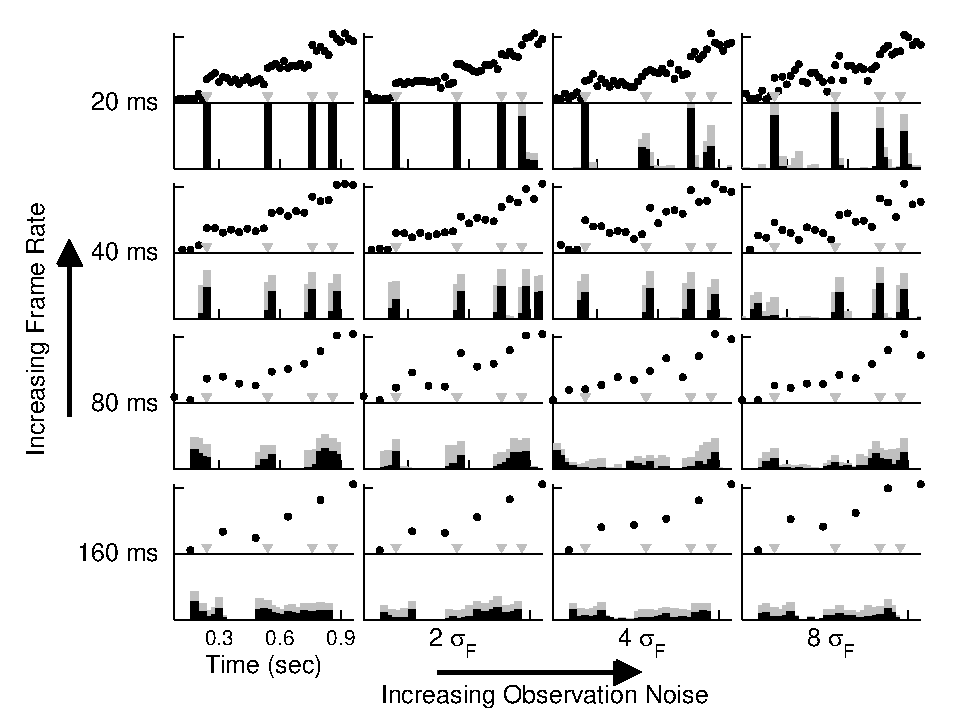
\includegraphics[width=1.0\linewidth]{ArraySim}
\caption{Array of inferences} \label{fig:array}
\end{figure}

\clearpage \newpage
\begin{figure}
\begin{centering}
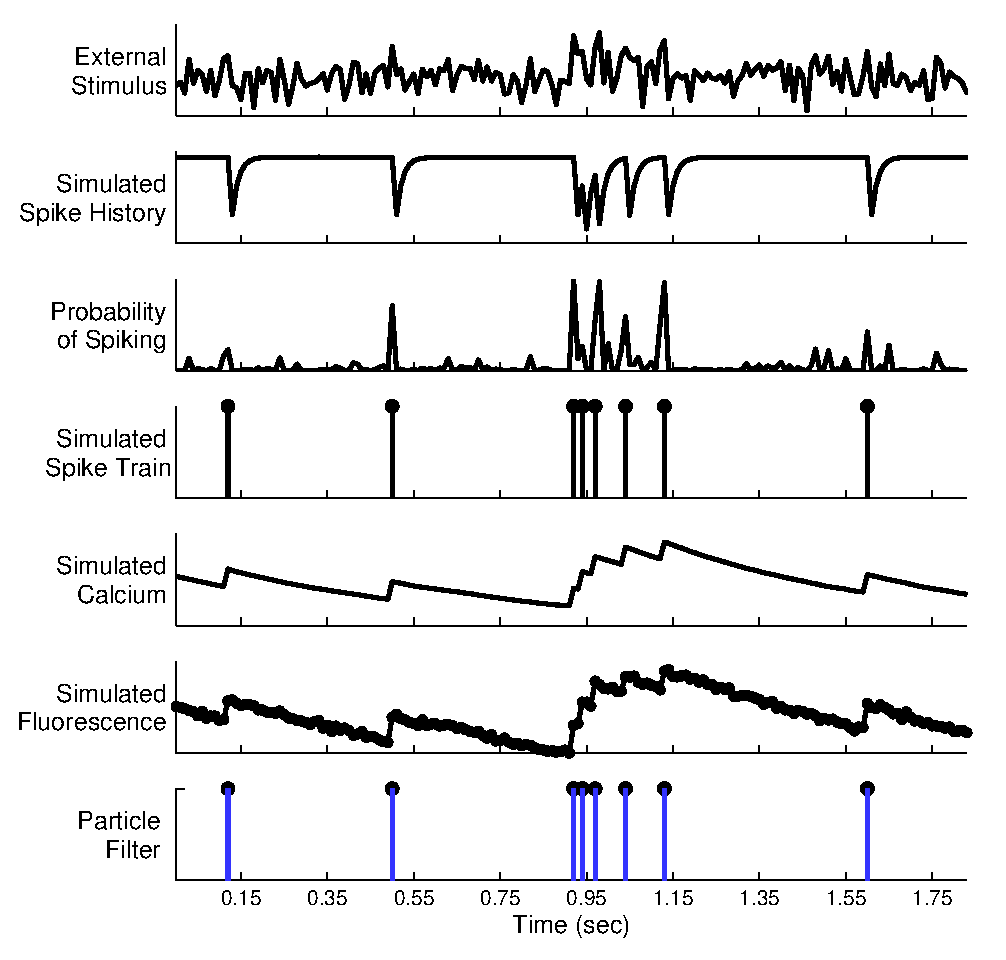
\includegraphics[width=1\linewidth]{StimSim}
\end{centering}
\caption{Superresolution simulation} \label{fig:StimSim}
\end{figure}

\clearpage \newpage
\begin{figure}
\includegraphics[width=1.0\linewidth]{StimData}
\caption{Real data superresolution} \label{fig:real}
\end{figure}

\clearpage \newpage
\begin{figure}
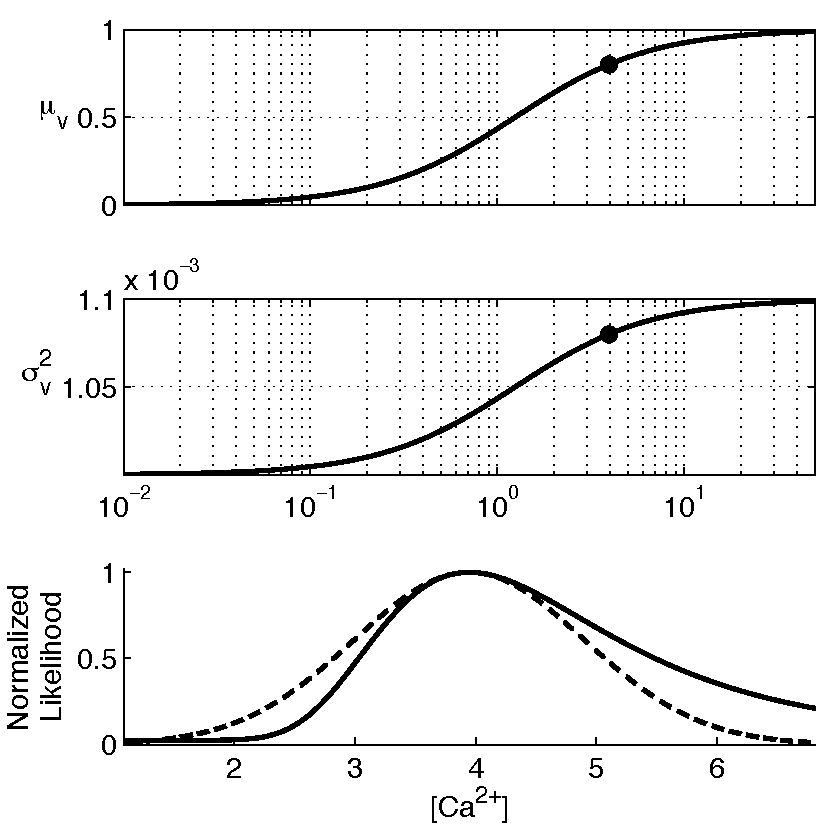
\includegraphics[width=\linewidth]{ca_nonlin}
\caption{Laplacian approximation of observation distribution} \label{fig:ca_nonlin}
\end{figure}

\clearpage \newpage
\begin{figure}
\centering \includegraphics[height=0.8\textheight]{sampl3}
\caption{The conditional sampler outperforms the prior sampler.} \label{fig:sampl}
\end{figure}

\clearpage \newpage
\begin{figure}
\centering
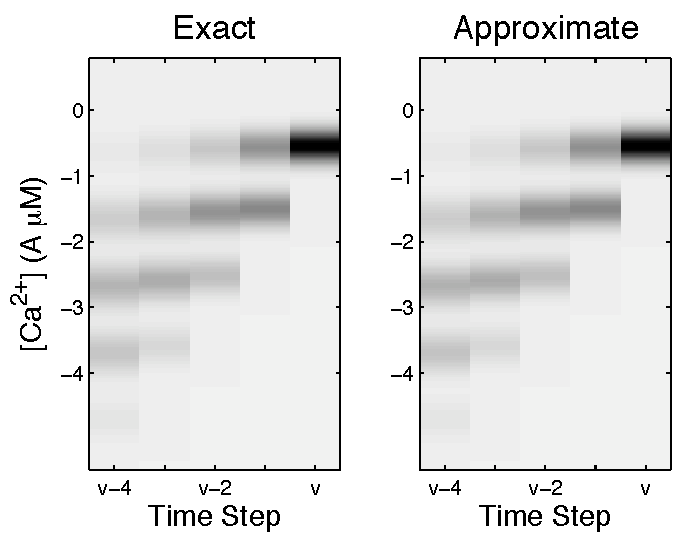
\includegraphics[width=0.5\linewidth]{PFapprox2}
\caption{Approximate distribution closely matches exact (analytical) distribution} \label{fig:pf2}
\end{figure}
\end{document} 
